\documentclass[reqno,12pt]{amsart}

\usepackage[colorlinks=true]{hyperref}
\hypersetup{urlcolor=blue, citecolor=red}

\usepackage{amssymb,graphicx,color}
\usepackage[latin1]{inputenc}

\usepackage[capitalize,nameinlink,noabbrev]{cleveref}

%The Layout
\setlength{\oddsidemargin}{0pt}
\setlength{\evensidemargin}{0pt}
\setlength{\textheight}{42\baselineskip}
\setlength{\textwidth}{6in}
%\addtolength{\headheight}{0.7in}

\theoremstyle{plain} % default style for the following 
\newtheorem{theorem}{Theorem}[section]
\newtheorem{lemma}{Lemma}[section]
\newtheorem{proposition}{Proposition}[section]
\newtheorem{corollary}{Corollary}[section]
%\newtheorem{definition}{Definition}[section]
\newtheorem{problem}{Problem}[section]
\newtheorem{stdhyp}{Standing Hypothesis}[section]
\theoremstyle{definition} % definition style for the following 
\newtheorem{remark}{Remark}[section]
\newtheorem{fact}{Fact}[section]

%\newcommand{\comment}[1]{\textcolor{red}{\framebox{\parbox{0.9\textwidth}{\textbf{#1}}}}}
\newcommand{\comment}[1]{\textcolor{red}{\textbf{#1}}}
\newcommand{\doshow}[1]{#1}
\newcommand{\dontshow}[1]{}
\newcommand{\extra}[1]{\dontshow{#1}} % use \show to show the extra stuff or \donotshow not to show it

%\mathchardef\mhyphen="2D

\renewcommand{\subjclassname}{$2020$ Mathematics Subject Classification}

\renewcommand{\theenumi}{\roman{enumi}}

\begin{document}
\numberwithin{equation}{section}

% Article info

\title[Strong convergence of the Euler method for Random ODEs]{Improved error estimate for the order of strong convergence of the Euler method for random ordinary differential equations}

\author[P. E. Kloeden]{Peter E. Kloeden}
\author[R. M. S. Rosa]{Ricardo M. S. Rosa}

\address[Peter E. Kloeden]{Mathematics Department, University of T\"ubingen, Germany}
\address[Ricardo M. S. Rosa]{Instituto de Matem\'atica, Universidade Federal do Rio de Janeiro, Brazil}

\email[P. E. Kloeden]{kloeden@math.uni-frankfurt.de}
\email[R. M. S. Rosa]{rrosa@im.ufrj.br}

\date{\today}

\thanks{The second author was partly supported by the Laborat\'orio de Matem\'atica Aplicada, Instituto de Matem\'atica, Universidade Federal do Rio de Janeiro (LabMA/IM/UFRJ)}

\makeatletter
\@namedef{subjclassname@2020}{\textup{2020} Mathematics Subject Classification}
\makeatother
\subjclass[2020]{60H35 (Primary), 65C30, 34F05 (Secondary)}
% 60H35 Computational methods for stochastic equations (aspects of stochastic analysis)
% 65C30 Numerical solutions to stochastic differential and integral equations
% 34F05: Equations and systems with randomnes; in 34Fxx: Equations and systems with randomness 
% 60H10: Stochastic ordinary differential equations; in 60Hxx: Stochastic analysis
% 65L20: Stability and convergence of numerical methods; in 65Lxx: Ordinary differential equations

\keywords{random ordinary differential equations, Euler method, strong convergence, It\^o process, point process, fractional Brownian motion}.

\begin{abstract}
It is well known that the Euler method for approximating the solutions of a random ordinary differential equation $\mathrm{d}X_t/\mathrm{d}t = f(t, X_t, Y_t)$ driven by a stochastic process $\{Y_t\}_t$ with $\theta$-H\"older sample paths is estimated to be of strong order $\theta$ with respect to the time step, provided $f=f(t, x, y)$ is sufficiently regular and with suitable bounds. This order increases to $1$ in some special cases, such as that of an It\^o diffusion noise. Here, it is proved that, in many more typical cases, further structures on the noise can be exploited so that the strong convergence is of order 1. This applies no only to It\^o process noises, but also to point-process noises, transport-type processes with sample paths of bounded variation, time-changed Brownian motion, and more generally to any noise that is a semi-martingale. The result follows from estimating the global error as an iterated integral over both large and small mesh scales, and then by switching the order of integration to move the critical regularity to the large scale. The work is complemented with numerical simulations illustrating the strong order 1 convergence in those cases, and with an example with fractional Brownian motion noise with Hurst parameter $0 < H < 1/2$ for which the order of convergence is $H + 1/2$, hence lower than the attained order 1 in the semi-martingale examples above, but still higher than the order $H$ of convergence expected from previous works.
\end{abstract}

\maketitle

\section{Introduction}

Consider the following initial value problem for a \textbf{random ordinary differential equation (RODE)}:
\begin{equation}
  \label{rodeeq}
  \begin{cases}
    \displaystyle \frac{\mathrm{d}X_t}{\mathrm{d} t} = f(t, X_t, Y_t), & 0 \leq t \leq T, \\
    \left. X_t \right|_{t = 0} = X_0,
  \end{cases}
\end{equation}
on a time interval $I=[0, T]$, with $T > 0$, and where the noise $\{Y_t\}_{t\in I}$ is a given stochastic process. This can be a scalar or a system of equations and the noise can also be either scalar or vector valued. The sample space is denoted by $\Omega$.

The Euler method for solving this initial value problem consists in approximating the solution on a uniform time mesh $t_j = j\Delta t_N$, $j = 0, \ldots, N$, with fixed time step $\Delta t_N = T/N$, for a given $N\in \mathbb{N}$. In such a mesh, the Euler scheme takes the form
\begin{equation}
  \label{emscheme}
  \begin{cases}
    X_{t_j}^N = X_{t_{j-1}}^N + \Delta t_N f(t_{j-1}, X_{t_{j-1}}^N, Y_{t_{j-1}}), & j = 1, \ldots, N, \\
    X_0^N = X_0.
  \end{cases}
\end{equation}
Notice $t_j = j\Delta t_N = jT/N$ also depends on $N$, but we do not make this dependency explicit, for the sake of notational simplicity.

We are interested in the order of \emph{strong} convergence, i.e. the approximation $\{X_{t_j}^N\}_j$ is said to converge to $\{X_t\}_t$ with \emph{strong order $\theta>0$} when there exists a constant $C \geq 0$ such that
\begin{equation}
    \label{strongordertheta}
    \max_{j=0, \ldots, N}\mathbb{E}\left[ \left\| X_{t_j} - X_{t_j}^N \right\| \right] \leq C \Delta t_N^\theta, \qquad \forall N \in \mathbb{N},
\end{equation}
where $\mathbb{E}[\cdot]$ indicates the expectation of a random variable on $\Omega$, and $\|\cdot\|$ is the norm in the appropriate phase space. There are other important notions of convergence, such as weak convergence, mean-square convergence, $p$-th mean convergence, and pathwise convergence (see e.g. \cite{HanKloeden2017,HighamKloeden2021, JentzenKloeden2011}), but we focus on strong convergence, here.

Under certain regularity conditions on $f$, it is proved in \cite[Theorem 3]{WangCaoHanKloeden2021} that, when the noise $\{Y_t\}_{t\in I}$ has $\theta$-H\"older continuous sample paths, the Euler scheme converges to the exact solution in the mean square sense with order $\theta$ with respect to the time step. This implies the strong convergence \eqref{strongordertheta} with the same order $\theta$. For pathwise convergence, see e.g. \cite{GruneKloeden2001,KloedenJentzen2007,JentzenKloeden2011,AsaiKloeden2016,HanKloeden2017}. In the case of fractional Brownian motion noise with Hurst parameter $H$, it is proved in \cite[Theorem 2]{WangCaoHanKloeden2021} that the mean square convergence is of order $H$.

In some particular cases, the order of convergence of the Euler method may be higher than the associated H\"older exponent of the noise, such as for Wiener process noises (see e.g. \cite[Example 5]{WangCaoHanKloeden2021}), but in general that would not be expected from previous results.

Our aim is to show, however, that, in many classical examples, it is possible to exploit further conditions that yield in fact a higher strong order of convergence, with the sample noise paths still being H\"older continuous or even discontinuous. This is the case, for instance, when the noise is a point process, a transport process, or an It\^o process, for which the convergence is of strong order 1. It is also the case for fractional Brownian motion noise with Hurst parameter $H$, for which the sample paths are $H$-H\"older continuous, but the strong convergence is of order 1, when $1/2 \leq H < 1$, and of order $H + 1/2$, when $0 < H < 1/2$.

The global condition on $f$ is a natural assumption when looking for strong convergence. Pathwise convergence, on the other hand, usually requires less stringent conditions (see e.g. \cite{JentzenKloedenNeuenkirch2009, JentzenKloeden2011}), but those are not the subject of interest here. The possibility of extending the improved order of strong convergence to pathwise convergence seems feasible for the case of sample paths of bounded variation but not so much for It\^o process noises for which the It\^o isometry is of fundamental importance. These will be investigated in a future oportunity.

The first main idea of the proof is to not estimate the local error and, instead, work with an explicit formula for the global error (see \cref{lemglobalerrorintegralformula}), similarly to the way it is done for approximations of stochastic differential equations, namely
\begin{equation}
    \label{lemglobalerrorintegralformulaintro}
    \begin{aligned}
        X_{t_j} - X_{t_j}^N & = X_0 - X_0^N + \int_0^{t_j} \left( f(s, X_s, Y_s) - f(s, X_{\tau^N(s)}, Y_s) \right)\;\mathrm{d}s  \\ 
        & \qquad + \int_{0}^{t_j} \left( f(s, X_{\tau^N(s)}, Y_s) - f(s, X_{\tau^N(s)}^N, Y_s) \right)\;\mathrm{d}s \\
        & \qquad + \int_0^{t_j} \left( f(s, X_{\tau^N(s)}^N, Y_s) - f(\tau^N(s), X_{\tau^N(s)}^N, Y_{\tau^N(s)}) \right)\;\mathrm{d}s,
    \end{aligned}
\end{equation}
for $j = 1, \ldots, N,$ where $\tau^N(t) = \max_{t_j \leq t} t_j$ is a piecewise constant function jumping to the mesh points $t_j$ (see \eqref{tauNt}).

The first term vanishes due to the initial condition $X_0^N = X_0$. The second term only depends on the solution and can be easily estimated with natural regularity conditions on the term $f=f(t, x, y)$. The third term is handled solely with the typical required condition on $f=f(t, x, y)$ of being globally Lipschitz continuous with respect to $x$. With those, we obtain the following basic bound for the global error (see \cref{lembasicestimate})
\begin{multline}
    \label{Etjbasicboundintro}
        \|X_{t_j} - X_{t_j}^N\| \leq \left( \|X_0 - X_0^N\| + L_X \int_0^{t_j} \|X_s - X_{\tau^N(s)}\| \;\mathrm{d}s \right. \\
        \left. \left\|\int_0^{t_j} \left( f(s, X_{\tau^N(s)}^N, Y_s) - f(\tau^N(s), X_{\tau^N(s)}^N, Y_{\tau^N(s)}) \right)\;\mathrm{d}s\right\|\right) e^{L_X t_j}.
\end{multline}

The only problematic, noise-sensitive term is the last one. The classical analysis is to use an assumed $\theta$-H\"older regularity of the noise sample paths and estimate the local error as
\[
    \mathbb{E}\left[\left\|f(s, X_{\tau^N(s)}^N, Y_s) - f(\tau^N(s), X_{\tau^N(s)}^N, Y_{\tau^N(s)})\right\|\right] \leq C\Delta t_N^{\theta}.
\]
Instead, we look at the whole noise error 
\[
    \mathbb{E}\left[\left\|\int_0^{t_j} \left( f(s, X_{\tau^N(s)}^N, Y_s) - f(\tau^N(s), X_{\tau^N(s)}^N, Y_{\tau^N(s)}) \right)\;\mathrm{d}s\right\|\right]
\]
and assume that the steps of the process given by $F_t = f(t, X_{\tau^N(t)}^N, Y_t)$ can be controlled in a suitable global way. In order to give the main idea, let us consider a scalar equation with a scalar noise and assume that the sample paths of $\{F_t\}_{t\in I}$ satisfy
\[
    F_s - F_\tau = \int_\tau^s \;\mathrm{d}F_\xi.
\]
For a semi-martingale noise, the integral above can be a combination of a Lebesgue-Stieltjes integral, a stochastic integral, and an integral with respect to a jump measure, but we leave it like that just for the sake of explaining the main idea. With that, we bound the global error term using the Fubini Theorem, taking into consideration that, despite the inner integral being from $\xi$ to the ``future'' $\tau^N(\xi) + \Delta t_N$, the integrand is still non-anticipative, 
\begin{multline*}
    \int_0^{t_j} \left( f(s, X_{\tau^N(s)}^N, Y_s) - f(\tau^N(s), X_{\tau^N(s)}^N, Y_{\tau^N(s)}) \right)\;\mathrm{d}s = \int_0^{t_j} \int_{\tau^N(s)}^s \;\mathrm{d}  F_\xi\;\mathrm{d}s \\
    = \int_0^{t_j} \int_{\xi}^{\tau^N(\xi) + \Delta t_N} \;\mathrm{d}s \;\mathrm{d} F_\xi  = \int_0^{t_j} (\tau^N(\xi) + \Delta t_N - \xi) \;\mathrm{d} F_\xi.
\end{multline*}
Then, since $0 \leq \tau^N(\xi) + \Delta t_N - \xi \leq \Delta t_N$, we find that
\begin{multline*}
    \mathbb{E}\left[\left\| \int_0^{t_j} \left( f(s, X_{\tau^N(s)}^N, Y_s) - f(\tau^N(s), X_{\tau^N(s)}^N, Y_{\tau^N(s)}) \right)\;\mathrm{d}s\right\|\right] \\
    \leq \Delta t_N\mathbb{E}\left[\left\| \int_0^{t_j} \;\mathrm{d} F_\xi \right\|\right].
\end{multline*}

We consider two types of noises, one whose paths are almost surely c\`adl\`ag (right continuous with left limits) with finite variation, and for which we prove the pathwise convergence of order 1, and more general semi-martingale noises, for which we prove the strong convergence of order 1.
These two cases are treated, respectively, in \cref{secmonotonicbound} and \cref{secsubmartingale}, with the main results in \cref{thmcadlagfv} and \cref{thmsemimartingale}.

We complement this work with a number of explicit examples and their numerical implementation, illustrating the strong order 1 convergence in the cases above. We include a system of linear equations with all sorts of noises, encompassing noises with sample paths with bounded variation and It\^o process noises. We also include an example with a fractional Brownian motion noise (fBm), for which the order of convergence drops to $H + 1/2$, when the Hurst parameter is in the range $0 < H < 1/2$. We do not present a general proof of this order of convergence in the case of fBm noise, but we prove it here in a particular linear equation. In this example, we essentially have (see \eqref{stepfBm} and \eqref{BHtintegralformulastep})
\[
    F_s - F_\tau \sim \int_\tau^s (s-\tau)^{H-1/2}\;\mathrm{d}W_\xi + \text{higher order term}.
\]
In this case, disregarding the higher order term,
\begin{align*}
    \int_0^{t_j} & \left( f(s, X_{\tau^N(s)}^N, Y_s) - f(\tau^N(s), X_{\tau^N(s)}^N, Y_{\tau^N(s)}) \right)\;\mathrm{d}s \\ 
    & \qquad \sim \int_0^{t_j} \int_{\tau^N(s)}^s (s-\tau^N(s))^{H-1/2} \;\mathrm{d} W_\xi\;\mathrm{d}s \\
    & \qquad = \int_0^{t_j} \int_{\xi}^{\tau^N(\xi) + \Delta t_N} (s-\tau^N(s))^{H-1/2} \;\mathrm{d}s \;\mathrm{d} W_\xi \\
    & \qquad \sim \int_0^{t_j} (\tau^N(\xi) + \Delta t_N - \tau^N(\xi))^{H+1/2} \;\mathrm{d} W_\xi \\
    & \qquad = (\Delta t_N)^{H+1/2} \int_0^{t_j} \;\mathrm{d} W_\xi.
\end{align*}
which, upon taking the expectation of the absolute value, yields a strong convergence of order $H + 1/2$.

Many other examples are included and also presented in more details in the github repository \cite{RODEConvEM2023}, such as a logistic model of population dynamics with random coefficients, loosely inspired by \cite[Section 15.2]{HanKloeden2017}, where the specific growth is the sine of a geometric Brownian motion process and with an extra point-process random term representing harvest; a toggle-switch model of gene expression (similar to \cite[Section 7.8]{Asai2016}, originated from \cite{VerdCrombachJaeger2014}, see also \cite{StrasserTheisMarr2012}) driven by a combination of a compound Poisson point process and an It\^o process, illustrating, again, the two main types of noises considered here; a mechanical structure model driven by a random disturbance simulating seismic ground-motion excitations in the form of a transport process, inspired by the Bogdanoff-Goldberg-Bernard model in \cite{BogdanoffGoldbergBernard1961} (see also \cite[Chapter 18]{NeckelRupp2013}, \cite{HousnerJenning1964}, and \cite{Kanai1957}, with this and other models, such as the ubiquotous Kanai-Tajimi and Clough-Penzien colored-noise models); an actuarial risk model for the surplus of an insurance company, inspired by \cite{GerberShiu1998} and \cite{BrigoMercurio2006}; and a Fisher-KPP partial differential equation with random boundary conditions, as inspired by the works of \cite{SalakoShen2020} and \cite{FreidlinWentzell1992} (see also \cite{Fisher1937} and \cite{KPP1937}), and where the noise is a colored noise modulated by a decaying self-exciting Hawkes point process.

\section{Pathwise solutions}
\label{secpathwisesolution}

For the notion and main results on pathwise solutions for RODEs, we refer the reader to \cite[Section 2.1]{HanKloeden2017} and \cite[Section 3.3]{NeckelRupp2013}.

We start with a fundamental set of conditions that imply the existence and uniqueness of pathwise solutions of the RODE \eqref{rodeeq} in the sense of Carath\'eodory:

\begin{stdhyp}
    \label{standinghypotheses1}
    We consider a function $f=f(t, x, y)$ defined on $I\times \mathbb{R}^d\times\mathbb{R}^k$ and with values in $\mathbb{R}^d$, and an $\mathbb{R}^k$-valued stochastic process $\{Y_t\}_{t\in I}$, where $I=[0, T]$, $T > 0$, and $d, k\in \mathbb{N}.$ We make the following standing assumptions:
    \begin{enumerate}
        \item \label{standinghypothesesLipschitzbound} The mapping $x \mapsto f(t, x, Y_t)$ is almost surely globally Lipschitz continuous on $x$, for every $t\in I$, with
        \begin{equation}
            \label{Ltassumptionbasic}
            \|f(t, x_1, Y_t) - f(t, x_2, Y_t)\| \leq L_t \|x_1 - x_2\|, \quad \forall t \in I, \;\forall x_1, x_2 \in\mathbb{R}^k,
        \end{equation}
        for a non-negative stochastic process $\{L_t\}_{t\in I}$ with Lebesgue integrable sample paths $t\mapsto L_t(\omega)$ on $I$.
        
        \item The mapping $t \mapsto f(t, x, Y_t(\omega))$ is Lebesgue measurable on $I$, for each $x\in \mathbb{R}^d$ and almost every sample path $t \mapsto Y_t(\omega)$;
        
        \item \label{standinghypothesesMbound} The bound $\|f(t, 0, Y_t)\| \leq M_t$ holds for all $t\in I$, where $\{M_t\}_{t\in I}$ is a non-negative stochastic process with Lebesgue integrable sample paths $t\mapsto M_t(\omega)$ on $I$.
    \end{enumerate}
\end{stdhyp}

Under these assumptions, for almost every sample value in $\Omega$, the integral equation
\begin{equation}
    \label{integralrodeform}
    X_t = X_0 + \int_0^t f(s, X_s, Y_s) \;\mathrm{d}s
\end{equation}
has a unique solution, in the Lebesgue sense, for the realizations $X_0 = X_0(\omega)$, of the initial condition, and $t\mapsto Y_t(\omega)$, of the noise process (see \cite[Theorem 1.1]{CoddingtonLevinson1985}). Moreover, the mapping $(t, \omega) \mapsto X_t(\omega)$ is measurable (see \cite[Section 2.1.2]{HanKloeden2017}) and, hence, give rise to a well-defined stochastic process $\{X_t\}_{t\in I}$.

Each pathwise solution of \eqref{integralrodeform} is absolutely continuous. From assumptions \eqref{standinghypothesesLipschitzbound} and \eqref{standinghypothesesMbound}, the solutions satisfy almost surely
\[
    \|X_t\| \leq \|X_0\| + \int_0^t (M_t + L_t\|X_t\|)\;\mathrm{d}s.
\]
Using Grownwall's inequality and the assumptions that $\{M_t\}_{t\in I}$ and $\{L_t\}_{t\in I}$ are integrable almost surely, it follows that
\begin{equation}
    \label{XtboundLXMt}
    \|X_t\| \leq \left(\|X_0\| + \int_0^t M_s\;\mathrm{d}s\right) e^{\int_0^t L_s\;\mathrm{d}s}, \quad \forall t\in I.
\end{equation}

More generally, since $t\mapsto X_t$ is absolutely continuous almost surely, we take the derivative of $\|X_t\|^\beta$ for an arbitrary power $\beta \geq 1$ to find that
\[
    \|X_t\|^\beta = \|X_0\|^\beta + q\int_0^t \|X_s\|^{\beta-2}X_s \cdot f(t, X_s, Y_s)\;\mathrm{d}s.
\]
Using again \eqref{standinghypothesesLipschitzbound} and \eqref{standinghypothesesMbound}, we obtain
\begin{align*}
    \|X_t\|^\beta & \leq \|X_0\|^\beta + \beta\int_0^t \|X_s\|^{\beta-1} \left(M_s + L_s \|X_s\|\right)\;\mathrm{d}s \\
    & \leq \|X_0\|^\beta + \beta\int_0^t \left(\frac{1}{\beta}M_s^\beta + \frac{\beta-1}{\beta}\|X_s\|^\beta + L_s \|X_s\|^\beta\right)\;\mathrm{d}s.
\end{align*}
By the Grownwall Lemma, the solutions satisfy almost surely
\begin{equation}
    \label{XtboundLXMtbeta}
    \|X_t\|^\beta \leq \left(\|X_0\|^\beta + \int_0^t M_s^\beta \;\mathrm{d}s\right) e^{\int_0^t \left(\beta - 1 + \beta L_s\right) \;\mathrm{d}s}.
\end{equation}

This is a useful pathwise estimate. For a strong norm estimate, though, we need to assume more, as illustrated by the following result.
\begin{lemma}
    Under the \cref{standinghypotheses1}, suppose further that
    \begin{equation}
        \label{EX0strongbound}
        \mathbb{E}[\|X_0\|] < \infty
    \end{equation}
    and
    \begin{equation}
        \label{EMtstrongbound}
        \int_0^T \mathbb{E}[M_s] \;\mathrm{d}s < \infty,
    \end{equation}
    and that $\{L_t\}_{t\in I}$ is essentially bounded, uniformly on $I$, i.e. there exists a constant $L_X > 0$ such that
    \begin{equation}
        \label{LtLXbound}
        L_t \leq L_X, \quad  t\in I,
    \end{equation}
    almost surely. Then
    \begin{equation}
        \label{EXtstrongbound}
        \mathbb{E}[\|X_t\|] \leq \left(\mathbb{E}[\|X_0\|] + \int_0^t \mathbb{E}[M_s]\;\mathrm{d}s\right) e^{L_X t}, \quad t\in I.
    \end{equation}
    If, moreover,
    \begin{equation}
        \label{EX0Mtstrongboundbeta}
        \mathbb{E}[\|X_0\|^\beta] < \infty, \quad
        \int_0^T \mathbb{E}[M_s^\beta] \;\mathrm{d}s < \infty,
    \end{equation}
    for a given $\beta \geq 1,$ then,
    \begin{equation}
        \label{EXtstrongboundbeta}
        \mathbb{E}[\|X_t\|^\beta] \leq \left(\mathbb{E}[\|X_0\|^\beta] + \int_0^t \mathbb{E}[M_s^\beta]\;\mathrm{d}s\right) e^{((\beta - 1) + \beta L_X) t}, \quad t\in I.
    \end{equation}
\end{lemma}

\begin{proof}
    Thanks to \eqref{XtboundLXMt} and \eqref{XtboundLXMtbeta}, the result is straightfoward.
\end{proof}

\begin{remark}
    When $f=f(t, x, y)$ is continuous on all three variables, as well as uniformly globally Lipschitz continuous in $x$, and the sample paths of $\{Y_t\}_{t\geq 0}$ are almost surely continuous, then the integrand in \eqref{integralrodeform} is almost surely continuous in $t$ and the integral becomes a Riemann integral. In this case, the integral form \eqref{integralrodeform} of the pathwise solutions of \eqref{rodeeq} holds in the Riemann sense.
\end{remark}

\begin{remark}
    In special \emph{dissipative} cases, depending on the structure of the equation, we might not need the second condition \eqref{EMtstrongbound} and only require $\mathbb{E}[\|X_0\|] < \infty$. More generally, when some bounded, positively invariant region exists and is of interest, we may truncate the nonlinear term to achieve the desired global conditions for the equation with the truncated term, but which coincides with the original equation in the region of interest. But we leave these cases to be handled in the applications, such as the population dynamics example in \cref{secpopdyn}.
\end{remark}

\section{Pathwise approximation}
\label{secpathwiseapproximation}

Similarly, under the \cref{standinghypotheses1}, we may obtain estimates for the Euler approximation \eqref{emscheme}. Notice that
\begin{align*}
    \|X_{t_j}^N\| & \leq \|X_{t_{j-1}}^N\| + \Delta t_N \|f(t_{j-1}, X_{t_{j-1}}^N, Y_{t_{j-1}})\| \\
    & \leq \|X_{t_{j-1}}^N\| + \Delta t_N (M_{t_{j-1}} + L_{t_{j-1}}\|X_{t_{j-1}}\|) \\
    & \leq \left(1 + L_{t_{j-1}}\Delta t_N\right)\|X_{t_{j-1}}^N\| + \Delta t_N M_{t_{j-1}}.
\end{align*}
We bound $(1 + a) \leq e^a$, so that
\[
    \|X_{t_j}^N\| \leq e^{L_{t_{j-1}}\Delta t_N}\|X_{t_{j-1}}^N\| + \Delta t_N M_{t_{j-1}}.
\]
Iterating this relation we obtain the bound
\begin{equation}
    \label{XNtboundLXMt}
    \|X_{t_j}^N\| \leq \left(\|X_0^N\| + \Delta t_N \sum_{i=0}^{j-1} M_{t_i}\right)e^{\Delta t_N \sum_{i=0}^{j-1} L_{t_i}}, \quad \forall j = 0, \ldots, N.
\end{equation}

\section{Integral formula for the global pathwise error}

In this section, we derive the following integral formula for the global error:
\begin{lemma}
    \label{lemglobalerrorintegralformula}
    Under the \cref{standinghypotheses1}, the Euler approximation \eqref{emscheme} for a pathwise solution of the random ordinary differential equation \eqref{rodeeq} satisfies almost surely the global error formula
    \begin{equation}
        \label{globalerrorintegralformula}
        \begin{aligned}
            X_{t_j} - X_{t_j}^N & = X_0 - X_0^N + \int_0^{t_j} \left( f(s, X_s, Y_s) - f(s, X_{\tau^N(s)}, Y_s) \right)\;\mathrm{d}s  \\ 
            & \qquad + \int_{0}^{t_j} \left( f(s, X_{\tau^N(s)}, Y_s) - f(s, X_{\tau^N(s)}^N, Y_s) \right)\;\mathrm{d}s \\
            & \qquad + \int_0^{t_j} \left( f(s, X_{\tau^N(s)}^N, Y_s) - f(\tau^N(s), X_{\tau^N(s)}^N, Y_{\tau^N(s)}) \right)\;\mathrm{d}s,
        \end{aligned}
    \end{equation}
    for $j = 1, \ldots, N,$ where $\tau^N$ is the piecewise constant jump function along the time mesh:
    \begin{equation}
        \label{tauNt}
        \tau^N(t) = \max_{t_j \leq t}\{t_j\} = \left[\frac{t}{\Delta t_N}\right]\Delta t_N = \left[\frac{tN}{T}\right]\frac{T}{N}.
    \end{equation}
\end{lemma}

\begin{proof}
    Under the \cref{standinghypotheses1}, the solutions of \eqref{rodeeq} are pathwise solutions in the Lebesgue sense of \eqref{integralrodeform}. With that in mind, we first obtain an expression for a single time step, from time $t_{j-1}$ to $t_j = t_{j-1} + \Delta t_N$.
    
    The exact pathwise solution satisfies
    $$
    X_{t_j} = X_{t_{j-1}} + \int_{t_{j-1}}^{t_j} f(s, X_s, Y_s) \;\mathrm{d}s.
    $$
    The Euler step is given by $X_{t_j}^N = X_{t_{j-1}}^N + \Delta t_N f(t_{j-1}, X_{t_{j-1}}^N, Y_{t_{j-1}}).$ Subtracting, we obtain
    $$
    X_{t_j} - X_{t_j}^N = X_{t_{j-1}} - X_{t_{j-1}}^N + \int_{t_{j-1}}^{t_j} \left( f(s, X_s, Y_s) - f(t, X_t^N, Y_t) \right)\;\mathrm{d}s.
    $$

    Adding and subtracting appropriate terms yield
    \begin{equation}
        \label{singlestep}
        \begin{aligned}
            X_{t_j} - X_{t_j}^N  = & X_{t_{j-1}} - X_{t_{j-1}}^N \\
            = &  \int_{t_{j-1}}^{t_j} \left( f(s, X_s, Y_s) - f(s, X_{t_{j-1}}, Y_s) \right)\;\mathrm{d}s \\ 
            & + \int_{t_{j-1}}^{t_j} \left( f(s, X_{t_{j-1}}, Y_s) - f(s, X_{t_{j-1}}^N, Y_s) \right)\;\mathrm{d}s \\
            & + \int_{t_{j-1}}^{t_j} \left( f(s, X_{t_{j-1}}^N, Y_s) - f(t_{j-1}, X_{t_{j-1}}^N, Y_{t_{j-1}}) \right)\;\mathrm{d}s.
        \end{aligned}
    \end{equation}

    Now we iterate the time steps \eqref{singlestep} to find that
    \begin{align*}
        X_{t_j} - X_{t_j}^N & = X_0 - X_0^N + \sum_{i=1}^{j} \left(\int_{t_{i-1}}^{t_i} \left( f(s, X_s, Y_s) - f(s, X_{t_{i}}, Y_s) \right)\;\mathrm{d}s \right. \\ 
        & \qquad + \int_{t_{i-1}}^{t_i} \left( f(s, X_{t_{i-1}}, Y_s) - f(s, X_{t_{i-1}}^N, Y_s) \right)\;\mathrm{d}s \\
        & \qquad \left. + \int_{t_{i-1}}^{t_i} \left( f(s, X_{t_{i-1}}^N, Y_s) - f(t_{i-1}, X_{t_{i-1}}^N, Y_{t_{i-1}}) \right)\;\mathrm{d}s \right).
    \end{align*}

    Using the jump function $\tau^N$ defined by \eqref{tauNt}, the above expression becomes \eqref{globalerrorintegralformula}.
\end{proof}

\section{Basic estimate for the global pathwise error}

Here we derive an estimate that is the basis for the specific estimates for each type of noise. For that, we use the following discrete version of the Grownwall Lemma, which is a particular case of the result found in \cite{GiraultRaviart1981} (see also \cite{Clark1987}). Its proof follows from \cite[Lemma V.2.4]{GiraultRaviart1981} by taking $n = j$, $a_n = e_j$, $b_n = 0$, $c_n = b$, and $\lambda = a$.

\begin{lemma}[Discrete Gronwall Lemma]
    \label{lemdiscretegronwall}
    Let $(e_j)_j$ be a (finite or infinite) sequence of positive numbers starting at $j=0$ and satisfying
    \begin{equation}
        \label{integralgronwall}
        e_j \leq \sum_{i=0}^{j-1} a_i e_i + b,
    \end{equation}
    for every $j$, with $e_0 = 0$, and where $a_i, b \geq 0$. Then,
    \begin{equation}
        \label{estimateintegralgronwall}
        e_j \leq b e^{\sum_{i=0}^{j-1} a_i}, \qquad \forall j.
    \end{equation}
\end{lemma}

We are now ready to start proving our basic estimate for the global pathwise error.
\begin{lemma}
    \label{lembasicestimate}
    Under the \cref{standinghypotheses1}, the global error \eqref{globalerrorintegralformula} is estimated as
    \begin{multline}
        \label{Etjbasicbound}
            \|X_{t_j} - X_{t_j}^N\| \leq \left( \|X_0 - X_0^N\| + \int_0^{t_j} L_s\|X_s - X_{\tau^N(s)}\| \;\mathrm{d}s \right. \\
            \left. \left\|\int_0^{t_j} \left( f(s, X_{\tau^N(s)}^N, Y_s) - f(\tau^N(s), X_{\tau^N(s)}^N, Y_{\tau^N(s)}) \right)\;\mathrm{d}s\right\|\right) e^{\int_0^{t_j} L_s\;\mathrm{d}s},
    \end{multline}
    for $j=1, \ldots, N$, where $\tau^N$ is given by \eqref{tauNt}.
\end{lemma}

\begin{proof}
    We estimate the first two integrals in \eqref{globalerrorintegralformula}. For the first one, we use \eqref{Ltassumptionbasic}, so that
    $$
        \|f(s, X_s, Y_s) - f(s, X_t, Y_s)\| \leq L_s \|X_s - X_t\|,
    $$
    for $t, s \in I$, and, in particular, for $t = \tau^N(s)$. Hence,
    $$
        \left\|\int_0^{t_j} \left( f(s, X_s, Y_s) - f(s, X_{\tau^N(s)}, Y_s) \right)\;\mathrm{d}s \right\| \leq \int_0^{t_j} L_s \|X_s - X_{\tau^N(s)}\| \;\mathrm{d}s.
    $$
    
    For the second term, we use again \eqref{Ltassumptionbasic}, so that
    $$
        \|f(s, X_t, Y_s) - f(s, X_t^N, Y_s)\| \leq L_s \|X_t - X_t^N\|,
    $$
    for any $t, s \in I$, and, in particular, for $t = \tau^N(s)$. Hence,
    \begin{multline*}
        \left\|\int_0^{t_j} \left( f(s, X_{\tau^N(s)}, Y_s) - f(s, X_{\tau^N(s)}^N, Y_s) \right)\;\mathrm{d}s \right\| \leq \int_0^{t_j} L_s \|X_{\tau^N(s)} - X_{\tau^N(s)}^N\| \;\mathrm{d}s \\
        \leq \sum_{i=0}^{j-1} \left(\int_{t_i}^{t_{i+1}}L_s\;\mathrm{d}s \right) \|X_{t_i} - X_{t_i}^N\|.
    \end{multline*}
    
    With these two estimates, we bound \eqref{globalerrorintegralformula} as
    \begin{align*}
        \|X_{t_j} - X_{t_j}^N\| & \leq \|X_0 - X_0^N\| + \int_0^{t_j} L_s \|X_s - X_{\tau^N(s)}\| \;\mathrm{d}s \\
        & \qquad + \sum_{i=0}^{j-1} \left(\int_{t_i}^{t_{i+1}}L_s\;\mathrm{d}s \right) \|X_{t_i} - X_{t_i}^N\| \\
        & \qquad + \left\|\int_0^{t_j} \left( f(s, X_{\tau^N(s)}^N, Y_s) - f(\tau^N(s), X_{\tau^N(s)}^N, Y_{\tau^N(s)}) \right)\;\mathrm{d}s\right\|.
    \end{align*}
    This can be cast in the form of \eqref{integralgronwall}. Then, using the discrete Gronwall \cref{lemdiscretegronwall}, we obtain \eqref{Etjbasicbound}.
\end{proof}

The first term in the right hand side of \eqref{Etjbasicbound} usually vanishes since in general we take $X_0^N = X_0$, but it suffices to assume that $X_0^N$ approximates $X_0$ to order $\Delta t_N$, which is useful for lower order approximations or for the discretization of (random) partial differential equations.

The third term in \eqref{Etjbasicbound} is the more delicate one that will be handled differently in the next sections.

As for the second term, which only concerns the solution itself, not the approximation, we use the following simple but useful general result.

\begin{lemma}
    \label{lemestimatesecondterminglobalerror}
    Under the \cref{standinghypotheses1} and assuming moreover that $t \mapsto L_t$ is bounded almost surely, we find that
    \begin{equation}
        \label{estimatesecondterminglobalerrorintegral}
        \int_0^{t_j}L_s\left\|X_s - X_{\tau^N(s)}\right\| \;\mathrm{d}s \leq \Delta t_N \left(\sup_{0\leq t \leq T} L_t \right)\int_0^{t_j} (M_s + L_s\|X_s\|) \;\mathrm{d}s.
    \end{equation}
\end{lemma}

\begin{proof}
    By assumptions \eqref{standinghypothesesLipschitzbound} and \eqref{standinghypothesesMbound} of the \cref{standinghypotheses1}, we have almost surely that
    \[
      \left\|X_s - X_{\tau^N(s)}\right\| = \left\|\int_{\tau^N(s)}^s f(\xi, X_\xi, Y_\xi)\;\mathrm{d}\xi\right\| \leq \int_{\tau^N(s)}^s (M_\xi + L_\xi\|X_\xi\|)\;\mathrm{d}\xi.
    \]
    Integrating over $[0, t_j]$ and using Fubini's theorem to exchange the order of integration,
    \begin{align*}
        \int_0^{t_j}L_s\left\|X_s - X_{\tau^N(s)}\right\| \;\mathrm{d}s & \leq \int_0^{t_j}L_s\int_{\tau^N(s)}^s (M_\xi + L_X\|X_\xi\|) \;\mathrm{d}\xi \;\mathrm{d}s \\
        & = \int_0^{t_j}(M_\xi + L_\xi\|X_\xi\|) \int_\xi^{\tau^N(\xi) + \Delta t_N} L_s\;\mathrm{d}s \;\mathrm{d}\xi.
    \end{align*}
    Using that $t \mapsto L_t$ is bounded almost surely, we find that
    \[
        \int_0^{t_j}L_s\left\|X_s - X_{\tau^N(s)}\right\| \;\mathrm{d}s \leq \int_0^{t_j} (\tau^N(\xi) + \Delta t_N - \xi) \left(\sup_{0\leq t \leq T} L_t \right)(M_\xi + L_s\|X_\xi\|) \;\mathrm{d}\xi
    \]
    Using that $\tau^N(\xi) \leq \xi$ and that the remaining terms are nonnegative, we have $\tau^N(\xi) + \Delta t_N - \xi \leq \Delta t_N,$ and we obtain exactly \eqref{estimatesecondterminglobalerrorintegral}.
\end{proof}

Combining the two previous results we obtain the following:

\begin{proposition}
    \label{propbasicestimate}
    Under the \cref{standinghypotheses1}, suppose further that \eqref{EX0strongbound}, \eqref{EMtstrongbound} and \eqref{LtLXbound} hold and that, for some constant $C_0 \geq 0$, 
    \begin{equation}
        \label{EX0X0N}
        \mathbb{E}[\|X_0 - X_0^N\|] \leq C_0 \Delta t_N, \qquad N\in \mathbb{N}.
    \end{equation}
    Then, for every $j = 0, \ldots, N$,
    \begin{multline}
        \label{expectedestimateglobalerrorintegral}
            \mathbb{E} \left[\|X_{t_j} - X_{t_j}^N\|\right] \leq \left( C_0 \Delta t_N + \Delta t_N L_X \left(\mathbb{E}[\|X_0\|] + \int_0^{t_j} \mathbb{E}[M_\xi]\;\mathrm{d}\xi\right)e^{L_X t_j}\right. \\
            \left. \mathbb{E}\left[\left\|\int_0^{t_j} \left( f(s, X_{\tau^N(s)}^N, Y_s) - f(\tau^N(s), X_{\tau^N(s)}^N, Y_{\tau^N(s)}) \right)\;\mathrm{d}s\right\|\right]\right) e^{L_X t_j}.
    \end{multline}
\end{proposition}

\begin{proof}
    Estimate \eqref{expectedestimateglobalerrorintegral} is obtained by taking the expectation of \eqref{Etjbasicbound} in \cref{lembasicestimate}, using the assumption \eqref{LtLXbound} to bound the exponential term, and properly estimating the first two terms inside the parentheses. The first term is handled with the assumption \eqref{EX0X0N}. We just need to take care of the second term.
    
    Under the \cref{standinghypotheses1}, together with \eqref{LtLXbound}, estimate \cref{lemestimatesecondterminglobalerror} applies and inequality \eqref{estimatesecondterminglobalerrorintegral} holds.
    Using \eqref{LtLXbound}, that inequality yields
    \[
        \int_0^{t_j} L_s \mathbb{E}[\|X_s - X_{\tau^N(s)}\|] \;\mathrm{d}s \leq \Delta t_N L_X \int_0^{t_j} (\mathbb{E}[M_s] + L_X\mathbb{E}[\|X_s\|]) \;\mathrm{d}s.
    \]
    Thanks to \eqref{EX0strongbound} and \eqref{EMtstrongbound}, inequality \eqref{EXtstrongbound} holds, and we obtain
    \begin{align*}
        \int_0^{t_j} & L_s \mathbb{E}[\|X_s - X_{\tau^N(s)}\|] \;\mathrm{d}s \\
        & \leq \Delta t_N L_X \int_0^{t_j} \left(\mathbb{E}[M_s] + L_X\left(\mathbb{E}[\|X_0\|] + \int_0^s \mathbb{E}[M_\xi]\;\mathrm{d}\xi\right)e^{L_X s} \right)\;\mathrm{d}s \\
        & \leq \Delta t_N L_X \left(\int_0^{t_j} \mathbb{E}[M_s] \;\mathrm{d}s + L_X \int_0^{t_j}\left(\mathbb{E}[\|X_0\|] + \int_0^{t_j} \mathbb{E}[M_\xi]\;\mathrm{d}\xi\right)e^{L_X s} \;\mathrm{d}s\right) \\
        & = \Delta t_N L_X \left(\int_0^{t_j} \mathbb{E}[M_s] \;\mathrm{d}s + \left(\mathbb{E}[\|X_0\|] + \int_0^{t_j} \mathbb{E}[M_\xi]\;\mathrm{d}\xi\right)\left(e^{L_X t_j} - 1\right) \right).
    \end{align*}
    Thus,
    \begin{equation}
        \label{expectedestimatesecondterminglobalerrorintegral}
        \int_0^{t_j} L_s \mathbb{E}[\|X_s - X_{\tau^N(s)}\|] \;\mathrm{d}s \leq \Delta t_N L_X \left(\mathbb{E}[\|X_0\|] + \int_0^{t_j} \mathbb{E}[M_\xi]\;\mathrm{d}\xi\right)e^{L_X t_j}.
    \end{equation}

    Now we look at \cref{lembasicestimate}. Taking the expectation of the global error formula \eqref{Etjbasicbound} and using \eqref{LtLXbound} to bound the exponential term, we arrive at
    \begin{multline*}
        \mathbb{E}\left[\|X_{t_j} - X_{t_j}^N\|\right] \leq \left( \mathbb{E}\left[\|X_0 - X_0^N\|\right] + \int_0^{t_j} L_s \mathbb{E}\left[\|X_s - X_{\tau^N(s)}\|\right] \;\mathrm{d}s \right. \\
        \left. \mathbb{E}\left[\left\|\int_0^{t_j} \left( f(s, X_{\tau^N(s)}^N, Y_s) - f(\tau^N(s), X_{\tau^N(s)}^N, Y_{\tau^N(s)}) \right)\;\mathrm{d}s\right\|\right]\right) e^{L_X t_j}.
    \end{multline*}
    Using now estimate \eqref{expectedestimatesecondterminglobalerrorintegral} and condition \eqref{EX0X0N}, we find \eqref{expectedestimateglobalerrorintegral}, completing the proof.
\end{proof}

\section{Pathwise convergence for noises with c\`adl\`ag sample paths of finite variation}
\label{secmonotonicbound}

Here, the noise $\{Y_t\}_{t\in I}$ is assumed to have sample paths that are c\`adl\`ag and with finite variation. By c\`adl\`ag we mean right continuous and with left limits (``continue \`a droite, limite \`a gauche", in French). More precisely, for almost every $\omega\in \Omega$, it is assumed that, for each $t\in I$, $\lim_{s\rightarrow t^+} Y_s(\omega) = Y_t(\omega)$ (right continuous); $\lim_{s \rightarrow t^-} Y_s(\omega)$ exists (left limits exist), and $V(\{Y_t\}_{t\in I}; I) = \sup_{t_0 < \ldots < t_n \in I, n\in \mathbb{N}} \sum_{i=1}^n \|Y_{t_i} - Y_{t_{i-1}}\| < \infty$ (finite variation). For such a process, we define the left-limit process
\begin{equation}
  Y_{t^{-}} = \lim_{t \rightarrow t^-} Y_s
\end{equation}
and the jump process
\begin{equation}
  \Delta Y_t = Y_t - Y_{t^{-}}.
\end{equation}
Almost surely, the sample paths of the jump process are constant except possibly at a countable number of points, denoted $J$, i.e. for almost every $\omega\in \Omega$, there exists a countable set $J(\omega) \subset I$ for which $\Delta Y_t(\omega)$ is constant on each connected component of $I\setminus J(\omega)$, and such that
\[
    \sum_{s\in J} \|\Delta Y_t\| \leq V(\{Y_t(\omega)\}_{t\in I}; I).
\]
In particular, for any given $\varepsilon > 0$, the set of times for which the jump $|\Delta Y_t|$ is larger than or equal to $\varepsilon$ is finite.

Given a continuously differentiable function $f:\mathbb{R}^k \rightarrow \mathbb{R}^k$, the following change of variables formula holds for such processes (see \cite[Theorems 31 and 33]{Protter2005}):
\begin{equation}
    f(Y_t) - f(Y_0) = \int_{0^+}^t Df(Y_{s^-}) \;\mathrm{d}Y_s + \sum_{0 < s \leq t} \left( f(Y_s) - f(Y_{s^{-}}) - Df(Y_{s^-})\Delta Y_s\right).
\end{equation}
The summation on the right hand side is an at most countable summation since the summand vanishes for $s \notin J$. The summation can be written as an integral with respect to a jump measure, but we keep it as a summation for simplicity.

The formula above is written in vectorial form, with $f$ and $Y_t$ of the form $f(y)=(f_i(y_1, \ldots, y_k))_{i=1, \ldots, k}$ and $Y_t = ((Y_t)_i)_{i=1, \ldots, k}$, and
\[
    Df(y)\Delta Y_t = \left( \nabla f_i(y)\Delta Y_t\right)_{i=1, \ldots, k} = \left( \sum_{j=1, \ldots, k} \partial y_j f_i(y) (Y_t)_j \right)_{i=1, \ldots, k}.
\]

When $f=f(t, y)$ depends also on $t$, one can apply the above formula to the extended process $\{(t, Y_t)\}_{t\in I}$. The first component is continuous hence has no jumps and the corresponding summation term vanishes. This leads to the following change of variables formula
\begin{multline}
    \label{changeofvariablesformulacadlagfv}
    f(t, Y_t) - f(0, Y_0) = \int_0^t \partial_s f(s, Y_{s^-})\;\mathrm{d}s + \int_{0^+}^t D_y f(s, Y_{s^-}) \;\mathrm{d}Y_s \\
    + \sum_{0 < s \leq t} \left( f(s, Y_s) - f(s, Y_{s^{-}}) - D_y f(s, Y_{s^-})\Delta Y_s\right).
\end{multline}
We actually apply this formula to a function of the form $f=f(t, x, y)$, but with $x$ constant, so the above formula suffices.

\begin{theorem}
    \label{thmcadlagfv}
    Under the \cref{standinghypotheses1}, suppose also that
    \begin{equation}
        \label{Ltboundedas}
        t \mapsto L_t \textrm{ is bounded almost surely};
    \end{equation}
    that 
    \begin{equation}
        \label{X0conv}
        \|X_0 - X_0^N\| \leq C_0\Delta t,
    \end{equation}
    for a random variable $C_0$ which is finite almost surely; and that $f=f(t, x, y)$ is uniformly globally Lipschitz continuous in $x$ and is continuously differentiable in $(t, y)$, with differentials $\partial_t f$ and $D_y f$ with at most linear growth in $x$, i.e.
    \begin{equation}
        \label{ftfylineargrowthcadlagfv}
        \left\|\partial_t f(t, x, y)\right\| \leq c_1 + c_2 \|x\| + c_3\|y\|, \quad \left\|D_y f(t, x, y)\right\| \leq c_4 + c_5\|x\| + c_6\|y\|,
    \end{equation}
    in $(t, x, y)\in I\times \mathbb{R}^d\times \mathbb{R}^k$, for suitable constants $c_1, c_2, c_3, c_4, c_5, c_6 \geq 0$. Assume, further, that the sample paths of $\{Y_t\}_{t\in I}$ are almost surely c\`adl\`ag with finite variation $V(\{Y_t\}_{t\in I}; I)$, on $I$. Then, the Euler scheme is pathwise convergent of order 1, i.e.
    \begin{equation}
        \label{ordercadlagfv}
        \max_{j=0, \ldots, N} \left\| X_{t_j}(\omega) - X_{t_j}^N(\omega) \right\| \leq C(\omega) \Delta t_N, \qquad \forall N \in \mathbb{N},
    \end{equation}
    for a suitable random variable $C$ which is finite almost surely.
\end{theorem}

\begin{proof}
    In view of \cref{lembasicestimate}, we need to estimate the last term of \eqref{Etjbasicbound}, namely
    \[
        \left\|\int_0^{t_j} \left( f(s, X_{\tau^N(s)}^N, Y_s) - f(\tau^N(s), X_{\tau^N(s)}^N, Y_{\tau^N(s)}) \right)\;\mathrm{d}s\right\|
    \]
    Thanks to \eqref{changeofvariablesformulacadlagfv}, we have
    \begin{align*}
        f(s, & X_{\tau^N(s)}^N, Y_s) - f(\tau^N(s), X_{\tau^N(s)}^N, Y_{\tau^N(s)}) = \int_{\tau^N(s)}^s D_\xi f(\xi, X_{\tau^N(s)}^N, Y_{\xi^-})\;\mathrm{d}\xi \\
        & + \int_{\tau^N(s)^+}^s D_y f(\xi, X_{\tau^N(s)}^N, Y_{\xi^-}) \;\mathrm{d}Y_\xi \\
        & + \sum_{\tau^N(s) < \xi \leq s} \left(f(\xi, X_{\tau^N(s)}^N, Y_\xi) - f(\xi, X_{\tau^N(s)}^N, Y_{\xi^{-}}) - D_y f(\xi, X_{\tau^N(s)}^N, Y_{\xi^-})\Delta Y_\xi\right).
    \end{align*}
    
    For the first term, we have, using \eqref{ftfylineargrowthcadlagfv},
    \begin{align*}
        & \left\|\int_0^{t_j} \int_{\tau^N(s)}^s D_\xi f(\xi, X_{\tau^N(s)}^N, Y_{\xi^-})\;\mathrm{d}\xi\;\mathrm{d}s\right\| \\
        & \qquad \leq \int_0^{t_j} \int_{\tau^N(s)}^s \left(c_1 + c_2 \|X_{\tau^N(s)}^N\| + c_3\|Y_{\xi^-}\|\right)\;\mathrm{d}\xi\;\mathrm{d}s.
    \end{align*}
    Exchanging the order of integration,
    \begin{align*}
        & \left\|\int_0^{t_j} \int_{\tau^N(s)}^s D_\xi f(\xi, X_{\tau^N(s)}^N, Y_{\xi^-})\;\mathrm{d}\xi\;\mathrm{d}s\right\| \\
        & \qquad \leq \int_0^{t_j} \int_{\xi}^{\tau^N(\xi) + \Delta t} \left(c_1 + c_2 \|X_{\tau^N(s)}^N\| + c_3\|Y_{\xi^-}\|\right)\;\mathrm{d}s\;\mathrm{d}\xi.
    \end{align*}
    For $s$ within $\xi \leq s < \tau^N(\xi) + \Delta t$, we have $\tau^N(s) = \tau^N(\xi)$. Moreover, $\tau^N(\xi) + \Delta t - \xi \leq \Delta t$. Hence
    \begin{align*}
        & \left\|\int_0^{t_j} \int_{\tau^N(s)}^s D_\xi f(\xi, X_{\tau^N(s)}^N, Y_{\xi^-})\;\mathrm{d}\xi\;\mathrm{d}s\right\| \\
        & \qquad \leq \int_0^{t_j} \int_{\xi}^{\tau^N(\xi) + \Delta t} \left(c_1 + c_2 \|X_{\tau^N(\xi)}^N\| + c_3\|Y_{\xi^-}\|\right)\;\mathrm{d}s\;\mathrm{d}\xi \\
        & \qquad \leq \Delta t\int_0^{t_j} \left(c_1 + c_2 \|X_{\tau^N(\xi)}^N\| + c_3\|Y_{\xi^-}\|\right)\;\mathrm{d}\xi.
    \end{align*}

    The second term is similar, except that now we integrate with respect to a finite variation process:
    \begin{align*}
        & \left\|\int_0^{t_j} \int_{\tau^N(s)^+}^s D_y f(\xi, X_{\tau^N(s)}^N, Y_{\xi^-}) \;\mathrm{d}Y_\xi\;\mathrm{d}s\right\| \\
        & \qquad \leq \int_0^{t_j} \int_{\tau^N(s)}^s \left(c_4 + c_5 \|X_{\tau^N(s)}^N\| + c_6\|Y_{\xi^-}\|\right)\;\|\mathrm{d}Y_\xi\|\;\mathrm{d}s \\
        & \qquad \leq \int_0^{t_j} \int_{\xi}^{\tau^N(\xi) + \Delta t} \left(c_4 + c_5 \|X_{\tau^N(s)}^N\| + c_6\|Y_{\xi^-}\|\right)\;\mathrm{d}s\;\|\mathrm{d}Y_\xi\| \\
        & \qquad \leq \Delta t \int_0^{t_j} \left(c_4 + c_5 \|X_{\tau^N(\xi)}^N\| + c_6\|Y_{\xi^-}\|\right)\;\|\mathrm{d}Y_\xi\|.
    \end{align*}

    For the third term, we have
    \begin{multline*}
        \left\|f(\xi, X_{\tau^N(s)}^N, Y_\xi) - f(\xi, X_{\tau^N(s)}^N, Y_{\xi^{-}}) - D_y f(\xi, X_{\tau^N(s)}^N, Y_{\xi^-})\Delta Y_\xi\right\| \\
        \leq 2(c_4 + c_5\|X_{\tau^N(s)}^N\| + c_6\max\{\|Y_{\xi^{-}}\|, \|Y_{\xi}\|)\})\|\Delta Y_\xi\|.
    \end{multline*}
    Hence,
    \begin{multline*}
        \left\|\int_0^{t_j} \sum_{\tau^N(s) < \xi \leq s} \left(f(\xi, X_{\tau^N(s)}^N, Y_\xi) - f(\xi, X_{\tau^N(s)}^N, Y_{\xi^{-}}) - D_y f(\xi, X_{\tau^N(s)}^N, Y_{\xi^-})\Delta Y_\xi\right)\;\mathrm{d}s\right\| \\
        \leq \int_0^{t_j} \sum_{\tau^N(s) < \xi \leq s} 2(c_4 + c_5\|X_{\tau^N(s)}^N\| + c_6\max\{\|Y_{\xi^{-}}\|, \|Y_{\xi}\|)\}\|\Delta Y_\xi\|\;\mathrm{d}s.
    \end{multline*}
    Switching the order of the integral and the summation, we find
    \begin{align*}
        & \left\|\int_0^{t_j} \sum_{\tau^N(s) < \xi \leq s} \left(f(\xi, X_{\tau^N(s)}^N, Y_\xi) - f(\xi, X_{\tau^N(s)}^N, Y_{\xi^{-}}) - D_y f(\xi, X_{\tau^N(s)}^N, Y_{\xi^-})\Delta Y_\xi\right)\;\mathrm{d}s\right\| \\
        & \qquad \leq \sum_{0 < \xi \leq t_j} \int_{\xi}^{\tau(\xi)+\Delta t} 2(c_4 + c_5\|X_{\tau^N(s)}^N\| + c_6\max\{\|Y_{\xi^{-}}\|, \|Y_{\xi}\|)\})\|\Delta Y_\xi\|\;\mathrm{d}s \\
        & \qquad \leq 2 \sum_{0 < \xi \leq t_j} \left(\int_{\xi}^{\tau(\xi)+\Delta t} (c_4 + c_5\|X_{\tau^N(s)}^N\| + c_6\max\{\|Y_{\xi^{-}}\|, \|Y_{\xi}\|)\}\;\mathrm{d}s \right)\|\Delta Y_\xi\| \\
        & \qquad \leq 2\left(c_4 + c_5\sup_{i=0, \ldots, j}\|X_i^N\| + c_6\sup_{0\leq s \leq t_j}\|Y_s\|\right) \Delta t \sum_{0 < \xi \leq t_j} \|\Delta Y_\xi\| \\
        & \qquad \leq 2\left(c_4 + c_5\sup_{i=0, \ldots, j}\|X_i^N\| + c_6\sup_{0\leq s \leq t_j}\|Y_s\|\right) V(\{Y_t\}_{t\in I}; [0, t_j]) \Delta t.
    \end{align*}
    Putting the estimates together, we find that
    \[
        \left\|\int_0^{t_j} \left( f(s, X_{\tau^N(s)}^N, Y_s) - f(\tau^N(s), X_{\tau^N(s)}^N, Y_{\tau^N(s)}) \right)\;\mathrm{d}s\right\| \leq \tilde C \Delta t,
    \]
    where $\tilde C$ is the random variable
    \begin{multline}
        \tilde C = \int_0^T \left(c_1 + c_2 \|X_{\tau^N(s)}^N\| + c_3\|Y_{s^-}\|\right)\;\mathrm{d}s \\
        + \int_0^T \left(c_4 + c_5 \|X_{\tau^N(s)}^N\| + c_6\|Y_{s^-}\|\right)\;\|\mathrm{d}Y_s\| \\
        + 2\left(c_4 + c_5\sup_{i=0, \ldots, N}\|X_i^N\| + c_6\sup_{0\leq s \leq T}\|Y_s\|\right) V(\{Y_t\}_{t\in I}; [0, t_j]).
    \end{multline}
    Using this estimate in \eqref{Etjbasicbound}, we obtain
    \[
        \|X_{t_j} - X_{t_j}^N\| \leq \left( \|X_0 - X_0^N\| + \int_0^{t_j} L_s\|X_s - X_{\tau^N(s)}\| \;\mathrm{d}s \right. \\
            \left. + \tilde C \Delta t\right) e^{\int_0^{t_j} L_s\;\mathrm{d}s}
    \]
    From \eqref{estimatesecondterminglobalerrorintegral} and the hypothesis \eqref{X0conv} on the initial condition we prove \eqref{ordercadlagfv}, with a suitable $C=C(\omega)$.
\end{proof}

\section{Strong converge for semi-martingale noises}
\label{secsubmartingale}

In the more general case of a semi-martingale noise $\{Y_t\}_{t\in I}$, the change of variables formula \eqref{changeofvariablesformulacadlagfv} takes the form (see \cite[Theorems 31 and 33]{Protter2005})
\begin{multline}
    \label{changeofvariablesformulasemimartingale}
    f(t, Y_t) - f(0, Y_0) = \int_0^t \partial_s f(s, Y_{s^-})\;\mathrm{d}s + \int_{0^+}^t D_y f(s, Y_{s^-}) \;\mathrm{d}Y_s \\
    + \sum_{0 < s \leq t} \left( f(s, Y_s) - f(s, Y_{s^{-}}) - D_y f(s, Y_{s^-})\Delta Y_s\right) \\
    + \frac{1}{2}\int_0^t D_{yy}f(s, Y_{s^-})\;\mathrm{d}[Y, Y]_t^c,
\end{multline}
where $\{[Y, Y]_t^c\}_{t\in I}$ is the continuous part of the quadratic variation process $\{[Y, Y]_t\}_{t\in I}$ defined by
\[
    [Y, Y]_t = Y_t^2 - 2\int_0^t Y_{t^-} \;\mathrm{d}Y_t.
\]
The quadratic variation is a c\'agl\'ag, increasing, and adapted process \cite[Theorem 22]{Protter2005}. The continuous part is given by
\[
    [Y, Y]_t^c = [Y, Y]_t - \sum_{0\leq s \leq t} \left(\Delta X_s\right)^2.
\]
Since $[Y, Y]_t^c$ is continuous and increasing, the corresponding integral is a Lebesgue-Stieltjes integral.

The Bichteler-Dellacherie Theorem \cite[Theorem 47]{Protter2005} which says that $\{Y_t\}_{t\in I}$, as any semi-martingale, can be decomposable in the form $Y_t = F_t + Z_t$, where $\{F_t\}_{t\in I}$ is an FV process (almost surely c\`adl\`ag paths of finite variation) and $\{Z_t\}_{t\in I}$ is a local martingale.

\begin{theorem}
    \label{thmsemimartingale}
    Under the \cref{standinghypotheses1}, suppose also that
    \begin{equation}
        t \mapsto L_t \textrm{ is bounded almost surely};
    \end{equation}
    that 
    \begin{equation}
        \mathbb{E}\left[\|X_0 - X_0^N\|\right] \leq c_0\Delta t,
    \end{equation}
    for a constant $c_0 \geq 0$; and that $f=f(t, x, y)$ is uniformly globally Lipschitz continuous in $x$ and is twice continuously differentiable in $(t, y)$, with partia differentials $\partial_t f$, $D_y f$ and $D_{yy} f$ satisfying
    \begin{equation}
        \label{ftfylineargrowthsemimartingale}
        \left\|\partial_t f(t, x, y)\right\| \leq c_1 + c_2 \|x\|, \;\; \left\|D_y f(t, x, y)\right\| \leq c_4 + c_5\|x\|, \;\; \left\|D_{yy} f(t, x, y)\right\| \leq c_7 + c_8\|x\|
    \end{equation}
    in $(t, x, y)\in I\times \mathbb{R}^d\times \mathbb{R}^k$, for suitable constants $c_1, c_2, c_4, c_5, c_7, c_8 \geq 0$. Assume, further, that $\{Y_t\}_{t\in I}$ is a semi-martingale. Then, the Euler scheme is strongly convergent of order 1, i.e.
    \begin{equation}
        \label{ordersemimartingale}
        \max_{j=0, \ldots, N} \mathbb{E}\left[\left\| X_{t_j} - X_{t_j}^N \right\|\right] \leq c \Delta t_N, \qquad \forall N \in \mathbb{N},
    \end{equation}
    for a suitable constant $c\geq 0$.
\end{theorem}

\begin{proof}
    As in the proof of \eqref{thmcadlagfv}, we need to estimate the last term of \eqref{Etjbasicbound}. Using \eqref{changeofvariablesformulasemimartingale}, the last term becomes
    \begin{align*}
        & \int_0^{t_j} \left( f(s, X_{\tau^N(s)}^N, Y_s) - f(\tau^N(s), X_{\tau^N(s)}^N, Y_{\tau^N(s)}) \right)\;\mathrm{d}s \\
        & = \int_0^{t_j} \int_{\tau^N(s)}^s D_\xi f(\xi, X_{\tau^N(s)}^N, Y_{\xi^-})\;\mathrm{d}\xi \;\mathrm{d}s \\
        & \quad + \int_0^{t_j} \int_{\tau^N(s)^+}^s D_y f(\xi, X_{\tau^N(s)}^N, Y_{\xi^-}) \;\mathrm{d}Y_\xi \;\mathrm{d}s \\
        & \quad + \int_0^{t_j} \sum_{\tau^N(s) < \xi \leq s} \left(f(\xi, X_{\tau^N(s)}^N, Y_\xi) - f(\xi, X_{\tau^N(s)}^N, Y_{\xi^{-}}) - D_y f(\xi, X_{\tau^N(s)}^N, Y_{\xi^-})\Delta Y_\xi\right) \;\mathrm{d}s \\ 
        & \quad + \frac{1}{2} \int_0^{t_j} \int_{\tau^N(s)}^s D_{yy}f(\xi, X_{\tau^N(s)}^N, Y_{\xi^-})\;\mathrm{d}[Y, Y]_\xi^c\;\mathrm{d}s.
    \end{align*}
    
    The first term is handled just like in the proof of \cref{thmcadlagfv} and we obtain
    \[
        \left\|\int_0^{t_j} \int_{\tau^N(s)}^s D_\xi f(\xi, X_{\tau^N(s)}^N, Y_{\xi^-})\;\mathrm{d}\xi\;\mathrm{d}s\right\| \leq \Delta t\int_0^{t_j} \left(c_1 + c_2 \|X_{\tau^N(\xi)}^N\|\right)\;\mathrm{d}\xi.
    \]

    For the second term, we use the Bichteler-Dellacherie Theorem \cite[Theorem 47]{Protter2005} which says that $\{Y_t\}_{t\in I}$, as any semi-martingale, can be decomposed in the form $Y_t = F_t + Z_t$, where $\{F_t\}_{t\in I}$ is an FV process (almost surely c\`adl\`ag paths of finite variation) and $\{Z_t\}_{t\in I}$ is a local martingale. Hence, the second term can be written as
    \begin{multline}
        \label{sm2}
        \int_0^{t_j} \int_{\tau^N(s)^+}^s D_y f(\xi, X_{\tau^N(s)}^N, Y_{\xi^-}) \;\mathrm{d}Y_\xi \;\mathrm{d}s = \int_0^{t_j} \int_{\tau^N(s)^+}^s D_y f(\xi, X_{\tau^N(s)}^N, Y_{\xi^-}) \;\mathrm{d}F_\xi \;\mathrm{d}s \\  
        + \int_0^{t_j} \int_{\tau^N(s)^+}^s D_y f(\xi, X_{\tau^N(s)}^N, Y_{\xi^-}) \;\mathrm{d}Z_\xi \;\mathrm{d}s,
    \end{multline}
    where the first inner integral is a Lebesgue-Stieltjes integral and the second inner integral is a stochastic integral with respect to a local martingale. Since $\{F_t\}_{t\in I}$ is of finite variation, the first part of \eqref{sm2} is estimated as in the proof of \cref{thmcadlagfv}, so that
    \begin{align*}
        & \left\|\int_0^{t_j} \int_{\tau^N(s)^+}^s D_y f(\xi, X_{\tau^N(s)}^N, Y_{\xi^-}) \;\mathrm{d}F_\xi\;\mathrm{d}s\right\| \\
        & \qquad \leq \int_0^{t_j} \int_{\tau^N(s)}^s \left(c_4 + c_5 \|X_{\tau^N(s)}^N\| + c_6\|Y_{\xi^-}\|\right)\;\|\mathrm{d}F_\xi\|\;\mathrm{d}s \\
        & \qquad \leq \int_0^{t_j} \int_{\xi}^{\tau^N(\xi) + \Delta t} \left(c_4 + c_5 \|X_{\tau^N(s)}^N\| + c_6\|Y_{\xi^-}\|\right)\;\mathrm{d}s\;\|\mathrm{d}F_\xi\| \\
        & \qquad \leq \Delta t \int_0^{t_j} \left(c_4 + c_5 \|X_{\tau^N(\xi)}^N\| + c_6\|Y_{\xi^-}\|\right)\;\|\mathrm{d}F_\xi\| \\
        & \qquad \leq \Delta t \left(c_4 + c_5 \max_{i=0, \ldots, j}\|X_{i}^N\| + c_6\sup_{0\leq \xi \leq t_j}\|Y_{\xi}\|\right)V(\{F_t\}_{t\in I}; [0, t_j]).
    \end{align*}
    For the second part of \eqref{sm2}, we use the It\^o isometry for local martingales, so that
    \begin{align*}
        & \mathbb{E}\left[\left\|\int_0^{t_j} \int_{\tau^N(s)^+}^s D_y f(\xi, X_{\tau^N(s)}^N, Y_{\xi^-}) \;\mathrm{d}Z_\xi\;\mathrm{d}s\right\|\right] \\
        & \quad = \mathbb{E}\left[\left\|\int_0^{t_j} \int_{\xi}^{\tau^N(\xi) + \Delta t} D_y f(\xi, X_{\tau^N(s)}^N, Y_{\xi^-}) \;\mathrm{d}s \;\mathrm{d}Z_\xi\right\|\right] \\
        & \quad \leq \mathbb{E}\left[\left(\int_0^{t_j} \int_{\xi}^{\tau^N(\xi) + \Delta t} D_y f(\xi, X_{\tau^N(s)}^N, Y_{\xi^-}) \;\mathrm{d}s \;\mathrm{d}Z_\xi\right)^2\right]^{1/2} \\
        & \quad \leq \mathbb{E}\left[\int_0^{t_j} \left(\int_{\xi}^{\tau^N(\xi) + \Delta t} \|D_y f(\xi, X_{\tau^N(s)}^N, Y_{\xi^-})\| \;\mathrm{d}s\right)^2 \;\mathrm{d}[Z_\xi, Z_\xi]\right]^{1/2} \\
        & \quad \leq \Delta t\mathbb{E}\left[\int_0^{t_j} \|D_y f(\xi, X_{\tau^N(\xi)}^N, Y_{\xi^-})\|^2 \;\mathrm{d}[Z_\xi, Z_\xi]\right]^{1/2}.
    \end{align*}

    The third term ... 

    The fourth and last term involves a Lebesgue-Stieltjes integral and is handled in a similar way, so that
    \begin{align*}
        & \left\|\frac{1}{2} \int_0^{t_j} \int_{\tau^N(s)}^s D_{yy}f(s, Y_{s^-})\;\mathrm{d}[Y, Y]_\xi^c\;\mathrm{d}s\right\| \\
        & \qquad \leq \frac{1}{2} \int_0^{t_j} \int_{\xi}^{\tau^N(\xi) + \Delta t} \left(c_1 + c_2 \|X_{\tau^N(\xi)}^N\|\right)\;\mathrm{d}s\;\mathrm{d}[Y, Y]_\xi^c \\
        & \qquad \leq \frac{\Delta t}{2}\int_0^{t_j} \left(c_1 + c_2 \|X_{\tau^N(\xi)}^N\|\right)\;\mathrm{d}[Y, Y]_\xi^c.
    \end{align*}
\end{proof}

\section{The case of an It\^o process noise}

Here, as explained in the Introduction, we assume the process given by $F_t = f(s, X_{\tau^N(s)}, Y_s)$ is an It\^o process, which, in applications, follows from the It\^o formula, assuming that $f=f(t, x, y)$ is sufficiently regular and that the noise $\{Y_t\}_{t\in I}$ is itself an It\^o process.

We recall (see e.g. \cite[Chapter 4]{Oksendal2003}) that an It\^o process is a process $\{Z_t\}_{t\in I}$ of the form
\begin{equation}
    \label{Itoprocess}
    \mathrm{d}Z_t = A_t\;\mathrm{d}t + B_t\;\mathrm{d}W_t.
\end{equation}
Here $Z_t$ can be either a scalar or a vector-valued process. In the scalar case, $\{W_t\}_{t\geq 0}$ is a (scalar) Wiener process, while $\{A_t\}_{t\in I}$ and $\{B_t\}_{t\in I}$ are real-valued processes adapted to $\{W_t\}_{t\geq 0}$.

In the vector-valued case, $\{A_t\}_{t\in I}$ is a vector-valued process with the same dimension as $Z_t$, while $\{B_t\}_{t\in I}$ is a square-matrix-valued process with the number of rows and of columns matching the dimension of $Z_t.$ The (multi-dimensional) Wiener process $\{W_t\}_{t\geq 0}$ is a vector-valued process $W_t = (W_t^{(j)})_j$ with the dimension matching the number of columns of $B_t$ and the dimension of $Z_t,$ and where each coordinate $\{W_t^{(j)}\}_{t\in I}$ is a Wiener process independent of the processes in the other coordinates. Both $\{A_t\}_{t\in I}$ and $\{B_t\}_{t\in I}$ are assumed to be adapted to each $\{W_t^{(j)}\}_{t\in I}.$ Writing the \emph{columns} of $B_t$ as $B_t^{(j)},$ we can write the stochastic term in \eqref{Itoprocess} as $B_t\;\mathrm{d}W_t = \sum_i B_t^{(j)}\;\mathrm{d}W_t^{(j)}.$ More explicitly, writing in full coordinates $Z_t = (Z_t^{(i)})_i,$ $A_t = (A_t^{(i)})_i,$ and $B_t = (B_t^{(i, j)})_{i, j},$ we have \eqref{Itoprocess} as the system
\begin{equation}
    \label{Itoprocesssystem}
    \mathrm{d}Z_t^{(i)} = A_t^{(i)}\;\mathrm{d}t + \sum_j B_t^{(i, j)}\;\mathrm{d}W_t^{(j)}, \quad \forall i.
\end{equation}

With that in mind, we first prove the following result.
\begin{lemma}
    \label{lemItostep}
    Besides the \cref{standinghypotheses1}, suppose that $F_t^N = f(t, X_{\tau^N(t)}^N, Y_t)$ is an It\^o process, i.e. satisfying \eqref{Itoprocess} with $Z_t = F_t^N$ and suitable processes $\{A_t\}_{t\in I}$ and $\{B_t\}_{t\in I}.$ Assume, moreover, that
    \begin{equation}
        \label{expectItostepterms}
        \int_0^T \mathbb{E}[\|A_t\|] \;\mathrm{d}t < \infty, \quad \int_0^T \mathbb{E}[\|B_t\|^2] \;\mathrm{d}t < \infty.
    \end{equation}
    Then,
    \begin{multline}
        \label{expectintfboundbyIto}
        \mathbb{E}\left[\left\|\int_0^t \left(f(s, X_{\tau^N(s)}^N, Y_s) - f(\tau^N(s), X_{\tau^N(s)}^N, Y_{\tau^N(s)})\right)\;\mathrm{d}s\right\|\right]  \\
        \leq \Delta t_N \left(\int_0^t \mathbb{E}[\|A_\xi\|] \;\mathrm{d}\xi + \left(\int_0^t \mathbb{E}[\|B_\xi\|^2] \;\mathrm{d}\xi \right)^{1/2}\right),
    \end{multline}
    for all $0 \leq t \leq T$ and every $N\in \mathbb{R}$.
\end{lemma}

\begin{proof}
    We write
    \[
        f(s, X_{\tau^N(s)}^N, Y_s) - f(\tau^N(s), X_{\tau^N(s)}^N, Y_{\tau^N(s)}) = \int_{\tau^N(s)}^s A_\xi \;\mathrm{d}\xi + \int_{\tau^N(s)}^s B_\xi \;\mathrm{d}W_\xi.
    \]
    Upon integration,
    \begin{multline*}
        \int_0^t \left(f(s, X_{\tau^N(s)}^N, Y_s) - f(\tau^N(s), X_{\tau^N(s)}^N, Y_{\tau^N(s)})\right)\;\mathrm{d}s  \\
        = \int_0^t \left(\int_{\tau^N(s)}^s A_\xi \;\mathrm{d}\xi + \int_{\tau^N(s)}^s B_\xi \;\mathrm{d}W_\xi\right)\;\mathrm{d}s.
    \end{multline*}
    Exchanging the order of integration, according to Fubini's theorem (see e.g. \cite[Section IV.6]{Protter2005} for a suitable stochastic version of the Fubini Theorem), yields
    \begin{align*}
        \int_0^t & \left(f(s, X_{\tau^N(s)}^N, Y_s) - f(\tau^N(s), X_{\tau^N(s)}^N, Y_{\tau^N(s)})\right)\;\mathrm{d}s \\
        & \qquad = \int_0^t \int_\xi^{\tau^N(\xi)+\Delta t_N} A_\xi \;\mathrm{d}s\;\mathrm{d}\xi + \int_0^t \int_\xi^{\tau^N(\xi) + \Delta t_N} B_\xi \;\mathrm{d}s\;\mathrm{d}W_\xi \\
        & \qquad = \int_0^t (\tau^N(\xi)+\Delta t_N - \xi) A_\xi \;\mathrm{d}\xi + \int_0^t (\tau^N(\xi) + \Delta t_N - \xi) B_\xi \;\mathrm{d}W_\xi.
    \end{align*}
    For exchanging the order of integration in the stochastic integral, an important aspect is that, although the integral in $s$ becomes an integral on the interval $[\xi, \tau^N(\xi) + \Delta t_N]$, which is posterior to $\xi$, the integrand does not depend on $s$ and, hence, does not violate any non-anticipative condition for the validity of the It\^o integral and of the stochastic Fubini Theorem.

    Taking the absolute mean and using the It\^o isometry \cite{Oksendal2003} on the second term give
    \begin{multline*}
        \mathbb{E}\left[\left\|\int_0^t \left(f(s, X_{\tau^N(s)}^N, Y_s) - f(\tau^N(s), X_{\tau^N(s)}^N, Y_{\tau^N(s)})\right)\;\mathrm{d}s\right\|\right]  \\
        \leq \int_0^t |\tau^N(\xi)+\Delta t_N - \xi| \mathbb{E}[\|A_\xi\|] \;\mathrm{d}\xi + \left(\int_0^t (\tau^N(\xi) + \Delta t_N - \xi)^2 \mathbb{E}[\|B_\xi\|^2] \;\mathrm{d}\xi \right)^{1/2}.
    \end{multline*}
    Since $|\tau^N(\xi)+\Delta t_N - \xi| \leq \Delta t_N$, we find
    \begin{multline*}
        \mathbb{E}\left[\left\|\int_0^t \left(f(s, X_{\tau^N(s)}^N, Y_s) - f(\tau^N(s), X_{\tau^N(s)}^N, Y_{\tau^N(s)})\right)\;\mathrm{d}s\right\|\right]  \\
        \leq \Delta t_N \left(\int_0^t \mathbb{E}[\|A_\xi\|] \;\mathrm{d}\xi + \left(\int_0^t \mathbb{E}[\|B_\xi\|^2] \;\mathrm{d}\xi \right)^{1/2}\right),
    \end{multline*}
    which completes the proof.
\end{proof}

Combining the estimate in \cref{lemItostep} with the estimate for the global error we obtain the following main result.
\begin{theorem}
    \label{thmItostep}
    Under the \cref{standinghypotheses1}, suppose also that
    \eqref{EX0strongbound}, \eqref{EMtstrongbound}, \eqref{EX0X0N}, \eqref{Itoprocess}, and \eqref{expectItostepterms} hold. Then, the Euler scheme \eqref{emscheme} is of strong order 1, i.e.
    \begin{equation}
      \label{Itosteptrongordernew}
        \max_{j=0, \ldots, N}\mathbb{E}\left[ \left\| X_{t_j} - X_{t_j}^N \right\| \right] \leq C \Delta t_N, \qquad \forall N \in \mathbb{N},
    \end{equation}
    for a constant $C$ given by
    \begin{multline}
        \label{constItostepboundstrongordernew}
        C = \left( C_0 +  L_X \left(\mathbb{E}[\|X_0\|] + \int_0^T \mathbb{E}[M_\xi]\;\mathrm{d}\xi\right)e^{L_X T}\right. \\
        \left. + \left(\int_0^T \mathbb{E}[\|A_\xi\|] \;\mathrm{d}\xi + \left(\int_0^T \mathbb{E}[\|B_\xi\|^2] \;\mathrm{d}\xi \right)^{1/2}\right)\right) e^{L_X T}.
    \end{multline}
\end{theorem}

\begin{proof}
    Under the \cref{standinghypotheses1}, the \cref{lembasicestimate} applies and the global error estimate \eqref{Etjbasicbound} holds. Thanks to \eqref{EX0strongbound}, \eqref{EMtstrongbound}, and \eqref{EX0X0N}, the \cref{propbasicestimate} applies and the global error is bounded according to \eqref{expectedestimateglobalerrorintegral}.
    
    With assumptions \eqref{Itoprocess} and \eqref{expectItostepterms}, the \cref{lemItostep} applies and the last term in \eqref{expectedestimateglobalerrorintegral} is bounded according to \eqref{expectintfboundbyIto}. Using \eqref{expectintfboundbyIto} in \eqref{expectedestimateglobalerrorintegral} yields
    \begin{multline*}
        \mathbb{E} \left[\left\|X_{t_j} - X_{t_j}^N\right\|\right] \leq \left( C_0 \Delta t_N + \Delta t_N L_X \left(\mathbb{E}[\|X_0\|] + \int_0^{t_j} \mathbb{E}[M_\xi]\;\mathrm{d}\xi\right)e^{L_X t_j}\right. \\
        \left. + \Delta t_N \left(\int_0^{t_j} \mathbb{E}[\|A_\xi\|] \;\mathrm{d}\xi + \left(\int_0^{t_j} \mathbb{E}[\|B_\xi\|^2] \;\mathrm{d}\xi \right)^{1/2}\right)\right) e^{L_X t_j}.
    \end{multline*}
    Since this holds for every $j=0, \ldots, N$, we obtain the desired estimate \eqref{Itosteptrongordernew}.
\end{proof}

In practice, conditions \eqref{Itoprocess}-\eqref{expectItostepterms} follow from assuming sufficent regularity on $f=f(t, x, y)$ and that the noise is an It\^o process. We assume the noise satisfies
\begin{equation}
    \label{YtItonoise}
    \mathrm{d}Y_t = a(t, Y_t)\;\mathrm{d}t + b(t, Y_t)\;\mathrm{d}W_t.
\end{equation}
In the scalar case ($k=1$), both $a=a(t, y)$ and $b=b(t, y)$ are scalars, while in the multi-dimensional case ($k > 1$), the coefficient $a = a(t, y) = (a_i(t, y))_i$ is vector valued with the same dimension $k$ as $y=(y_i)_i,$ and $b=b(t, y) = (b_{ij}(t, y))_{ij}$ is matrix valued, with dimension $k\times k$.

Then, we have following result.
\begin{theorem}
    \label{thmItonoise}
    Let $f=f(t, x, y)$ be twice continuously differentiable with uniformly bounded derivatives. Suppose that the noise $\{Y_t\}_{t\in I}$ is an It\^o process, satisfying \eqref{YtItonoise}, with $a=a(t, y)$ and $b=b(t, y)$ continuous and such that
    \begin{equation}
        \label{Itonoiseterms}
        \|a(t, y)\| \leq A_M + A_Y \|y\|, \qquad \|b(t, y)\| \leq B_M + B_Y\|y\|,
    \end{equation}
    for all $y,$ with constants $A_M, A_Y, B_M, B_Y \geq 0$.
    Assume the bounds \eqref{EX0strongbound} and \eqref{EX0X0N} hold, and that
    \begin{equation}
        \label{YtItonoiseinitialcondition}
        \mathbb{E}[\|Y_0\|] < \infty.
    \end{equation}
    Then, the Euler scheme is of strong order 1, i.e.
    \begin{equation}
        \max_{j=0, \ldots, N}\mathbb{E}\left[ \left\| X_{t_j} - X_{t_j}^N \right\| \right] \leq C \Delta t_N, \qquad \forall N \in \mathbb{N},
    \end{equation}
  for a suitable constant $C \geq 0$.
\end{theorem}

\begin{proof}
    Let us start by showing that the \cref{standinghypotheses1} is valid. Since $f=f(t, x, y)$ is (twice) continuously differentiable with, in particular, bounded derivative in $x$, then it is uniformly globally Lipschitz in $x$. Since $a=a(t, y)$ and $b=b(t, y)$ are continuous, the noise has continuous sample paths, almost surely. Thus, the remaining condition in the \cref{standinghypotheses1} to be verified is \eqref{standinghypothesesMbound}.

    Using the It\^o formula with \eqref{YtItonoise} in mind (see \cite[Theorem 4.1.2]{Oksendal2003} or \cite[Section 7.4]{Kuo2006} for the scalar case of the It\^o formula, with $g(t, y) = y^2,$ and \cite[Theorem 4.2.1]{Oksendal2003} or, more generally, \cite[Section 7.5]{Kuo2006} for the multi-dimensional case, with $g(t, y) = \|y\|^2$), we have
    \[
        \mathrm{d}\|Y_t\|^2 = \left(2a(t, Y_t) \cdot Y_t  + b(t, Y_t)^2 \right) \;\mathrm{d}t + 2b(t, Y_t) Y_t\;\mathrm{d}W_t.
    \]
    Thus,
    \[
        \|Y_t\|^2 = \|Y_0^2\| + \int_0^t \left(2a(s, Y_s)\cdot Y_s  + b(t, Y_s)^2 \right) \;\mathrm{d}s + \int_0^t 2b(s, Y_s) Y_s\;\mathrm{d}W_s.
    \]
    Taking the expectation,
    \[
        \mathbb{E}[\|Y_t\|^2] = \mathbb{E}[\|Y_0\|^2] + \int_0^t \mathbb{E}\left[\left(2a(s, Y_s) \cdot Y_s  + b(t, Y_s)^2 \right)\right] \;\mathrm{d}s.
    \]

    Using \eqref{Itonoiseterms}, this yields
    \begin{align*}
        \mathbb{E}[\|Y_t\|^2] & \leq \mathbb{E}[\|Y_0\|^2] + \int_0^t \left(2\mathbb{E}[(A_M + A_Y \|Y_s\|) \|Y_s\|]  + \mathbb{E}[(B_M + B_Y\|Y_s\|)^2] \right) \;\mathrm{d}s \\
        & \leq \mathbb{E}[\|Y_0\|^2] + \int_0^t \left((A_M^2 + (1 + 2A_Y) \mathbb{E}[\|Y_s\|^2])  + 2(B_M^2 + B_Y^2\mathbb{E}[\|Y_s\|^2]) \right) \;\mathrm{d}s.
    \end{align*}
    By the classical Gronwall Lemma \cite{Gronwall1919},
    \[
        \mathbb{E}[\|Y_t\|^2] \leq \left( \mathbb{E}[\|Y_0\|^2] + (A_M^2 + 2B_M^2)t\right)e^{(1 + 2A_Y + 2B_Y^2)t}.
    \]
    Thus,
    \begin{equation}
        \label{unifboundYtIto}
        \sup_{t\in I}\mathbb{E}[\|Y_t\|^2] \leq \left( \mathbb{E}[\|Y_0\|^2] + (A_M^2 + 2B_M^2)T\right)e^{(1 + 2A_Y + 2B_Y^2)T}.
    \end{equation}

    Since $f=f(t, x, y)$ is Lipschitz in $x$ and twice continuously differentiable in $(t, y)$ with uniformly bounded first order derivatives, we have the bound
    \[
        \|f(t, x, y)\| \leq \|f(0, 0, 0)\| + L_X\|x\| + L_T t + L_Y\|y\|.
    \]
    Thus,
    \[
        \|f(t, x, Y_t)\| \leq M_t + L_X\|x\|,
    \]
    with
    \[
        M_t = \|f(0, 0, 0)\| + L_T t + L_Y\|y\|.
    \]
    Thanks to \eqref{unifboundYtIto}, we see that
    \[
        \int_0^T M_t\;\mathrm{d}t < \infty.
    \]
    Therefore, we are under the conditions of the \cref{standinghypotheses1}.

    Now, in view of \cref{thmItostep}, it remains to prove that $F_t^N = f(t, X_{\tau^N(t)}^N, Y_t)$ is an It\^o process \eqref{Itoprocess}, with the bounds \eqref{expectItostepterms}. The fact that it is an It\^o process follows from the It\^o formula and the smoothness of $f=f(t, x, y)$, as we shall see now. We first consider the case of a scalar noise, for the sake of clarity. Since $(t, y) \mapsto f(t, x, y)$ is twice continuously differentiable, for each fixed $x$, the It\^o formula is applicable and yields, in the case of a scalar noise,
    \begin{multline}
        \label{itoformula}
        \mathrm{d}f(t, x, Y_t) = \left(\partial_t f(t, x, Y_t) + a(t, Y_t) \partial_y f(t, x, Y_t)  + \frac{b(t, Y_t)^2}{2}\partial_{yy}f(t, x, Y_t) \right) \;\mathrm{d}t \\ + b(t, Y_t) \partial_y f(t, x, Y_t)\;\mathrm{d}W_t,
    \end{multline}
    for every fixed $x\in \mathbb{R}$. This means \eqref{Itoprocess} holds with
    \[
        A_t = \partial_t f(t, x, Y_t) + a(t, Y_t) \partial_y f(t, x, Y_t)  + \frac{b(t, Y_t)^2}{2}\partial_{yy}f(t, x, Y_t)
    \]
    and
    \[
        B_t = b(t, Y_t) \partial_y f(t, x, Y_t).
    \]
    For the integrability conditions, since $f=f(t, x, y)$ has uniformly bounded derivatives, we have
    \[
        \|A_t\| \leq L_T + L_Y(A_M + A_Y\|Y_t\|) + 2L_{YY}(B_M^2 + B_Y^2\|Y_t\|^2),
    \]
    and
    \[
        \|B_t\| \leq L_Y (B_M + B_Y \|Y_t\|),
    \]
    for a suitable constant $L_{YY}\geq 0$. Now, thanks to \eqref{unifboundYtIto}, we see that \eqref{expectItostepterms} is satisfied.

    In the case of a multi-dimensional noise, we have $a(t, y) = (a_i(t, y))_i$ and $b(t, y) = (b_{ij}(t, y))_{ij},$ and \eqref{itoformula} becomes
    \begin{multline}
        \label{itoformulamulti}
        \mathrm{d}f(t, x, Y_t) = \left(\partial_t f(t, x, Y_t) + \sum_i \partial_{y_i} f(t, x, Y_t) a_i(t, Y_t) \right. \\
        \left. + \frac{1}{2}\sum_i \partial_{y_i}^2 f(t, x, Y_t)b_{ii}(t, Y_t)^2 \right) \;\mathrm{d}t \\ + \sum_{i,j}\partial_{y_i} f(t, x, Y_t) b_{ij}(t, Y_t) \;\mathrm{d}W_t^{(j)},
    \end{multline}
    so that \eqref{Itoprocess}/\eqref{Itoprocesssystem} and \eqref{expectItostepterms} follow similarly.

    Therefore, all the conditions of \cref{thmItostep} are met and we obtain the strong order 1 convergence of the Euler method.
\end{proof}

\begin{remark}
    When the diffusion coefficient $b = b(t, y) = b(t)$ in \eqref{YtItonoise} is independent of $y$, the noise is an additive noise, and in this case the Euler scheme is well known to be of strong order 1 \cite[Section 19.3.1]{HighamKloeden2021}. In the more general case $b=b(t, y)$, however, the Euler scheme has always been regarded to be of order 1/2 \cite{GruneKloeden2001} (see also \cite{WangCaoHanKloeden2021} for mean square convergence). Here, though, we deduce, under the conditions of \cref{thmItonoise}, that even if $b=b(t, y)$ depends on $y$, the strong convergence of the Euler scheme is actually of order 1.    
\end{remark}

\section{Numerical examples}
\label{secnumericalexamples}

In this section, we illustrate the improved order of convergence with several examples that fall into one of the cases considered above. We start with some linear equations, including all sorts of noises. Then we illustrate the $H + 1/2$ order of convergence in the case of a fractional Brownian motion (fBm) noise with Hurst parameter $0 < H < 1/2$. Next we move to a number of linear and nonlinear models, as mentioned in the Introduction. Details of the numerical implementations, with the full working code for reproducibility puposes is available in the github repository \cite{RODEConvEM2023}.

For estimating the order of convergence, we use the Monte Carlo method, computing a number of numerical approximations $\{X_{t_j}^N(\omega_m)\}_{j=0, \ldots, N}$, of sample path solutions $\{X_t(\omega_m)\}_{t\in I}$, for samples $\omega_m,$ with $m = 1, \ldots, M$, and taking the maximum in time of the average of their absolute differences at the mesh points:
\begin{equation}
    \epsilon^N = \max_{j=0, \ldots, N} \frac{1}{M}\sum_{m=1}^M \left|X_{t_j}(\omega_m) - X_{t_j}^N(\omega_m)\right|.
\end{equation}
Then we fit the errors $\epsilon^N$ to the power law $C\Delta t_N^p$, in order to find $p$, along with the 95\% confidence interval.

Here are the main parameters for the error estimate:
\begin{enumerate}
    \item The number $M\in\mathbb{N}$ of samples for the Monte Carlo estimate of the strong error.
    \item The time interval $[0, T], $ $T > 0,$ for the initial-value problem.
    \item The distribution law for the random initial condition $X_0$.
    \item A series of time steps $\Delta t_{N_i} = T/N_i$, with $N_i=2^{n_i},$ for some $n_i\in\mathbb{N},$ so that finer meshes are refinements of coarser meshes.
    \item A number $N_{\mathrm{tgt}}$ for a finer resolution to compute a target solution path, typically $N_{\mathrm{tgt}} = \max_i\{N_i^2\}$, unless an exact pathwise solution is available, in which case a coarser mesh of the order of $\max_i\{N_i\}$ can be used.
\end{enumerate}

And here is the method:
\begin{enumerate}
    \item For each sample $\omega_m,$ $m=1, \ldots, M$, we first generate a discretization of a sample path of the noise, $\{Y_{t_j}\}_{j=0, \ldots, N_{\mathrm{tgt}}},$ on the finest grid $t_j = j \Delta t_{N_{\textrm{tgt}}}$, $j = 0, \ldots, N_{\mathrm{tgt}},$ using an exact distribution for the noise.
    \item Next, we use the values of the noise at the target time mesh to generate the target solution $\{X_{t_j}\}_{j=0, \ldots, N_{\mathrm{tgt}}}$, still on the fine mesh. This is constructed either using the Euler approximation itself, keeping in mind that the mesh is sufficiently fine, or an exact distributions of the solution, when available.
    \item Then, for each time resolution $N_i,$ we compute the Euler approximation using the computed noise values at the corresponding coarser mesh $t_j = j\Delta t_{N_i},$ $j=0, \ldots, N_i.$
    \item We then compare each approximation $\{X_{t_j}^{N_i}\}_{j=0, \ldots, N_i}$ to the values of the target path on that coarse mesh and update the strong error
    \[
        \epsilon_{t_j}^{N_i} = \frac{1}{M}\sum_{m=1}^M \left|X_{t_j}(\omega_m) - X_{t_j}^{N_i}(\omega_m)\right|,
    \]
    at each mesh point.
    \item At the end of all the simulations, we take the maximum in time, on each corresponding coarse mesh, to obtain the error for each mesh,
    \[
        \epsilon^{N_i} = \max_{j=0, \ldots, N_i} \epsilon_{t_j}^{N_i}.
    \]
    \item We fit $(\Delta t_{N_i}, \epsilon^{N_i})$ to the power law $C\Delta t_{N_i}^p$, via linear least-square regression in log scale, so that $\ln \epsilon^{N_i} \sim \ln C + p \ln \Delta t_{N_i}$, for suitable $C$ and $p$, with $p$ giving the order of convergence. This amounts to solving the normal equation $(A^tA)\mathbf{v} = A^t\ln(\boldsymbol{\epsilon})$, where $\mathbf{v}$ is the vector $\mathbf{v} = (\ln(C), p)$, $A$ is the Vandermonde matrix associated with the logarithm of the mesh steps $(\Delta t_{N_i})_i$, and $\ln(\boldsymbol{\epsilon})$ is the vector $\ln(\boldsymbol{\epsilon}) = (\ln(\epsilon^{N_i}))_i$.
    \item We also compute the standard error of the Monte-Carlo sample at each time step,
    \[
        s_{t_j}^{N_i} = \frac{\sigma_{t_j}^{N_i}}{\sqrt{M}},
    \]
    where $\sigma_{t_j}^{N_i}$ is the sample standard deviation given by
    \[
        \sigma_{t_j}^{N_i} = \sqrt{\frac{1}{M-1}\sum_{m=1}^M \left(\left|X_{t_j}(\omega_m) - X_{t_j}^{N_i}(\omega_m) \right|- \epsilon_{t_j}^{N_i}\right)^2},
    \]
    and compute the 95\% confidence interval $[\epsilon_{\min}, \epsilon_{\max}]$ for the strong error with
    \[
        \epsilon_{\min}^{N_i} = \max_{j=0, \ldots, N_i} (\epsilon_{t_j}^{N_i} - 2\sigma_{t_j}^{N_i}), \quad \epsilon_{\max}^{N_i} = \max_{j=0, \ldots, N_i} (\epsilon_{t_j}^{N_i} + 2\sigma_{t_j}^{N_i}).
    \]
    \item Finally, from the normal equations above, we compute the 95\% confidence interval $[p_{\min}, p_{\max}]$ by computing the minimum and maximum values of $p$ in the image, by the linear map $\mathbf{e} \mapsto (\ln(C), p) = (A^tA)^{-1}A^t\ln(\mathbf{e})$, of the polytope formed by all combinations of the indices in $(\epsilon_{\min}^{N_i})_i$ and $(\epsilon_{\max}^{N_i})_i$, which is the image of the set of 95\% confidence intervals for the errors obtained with the Monte-Carlo approximation of the strong error.
\end{enumerate}

As for the implementation itself, all code is written in the Julia language \cite{Julia2017}. Julia is a high-performance programming language, suitable for scientific computing and computationally-demanding applications.

Julia has a feature-rich \texttt{DifferentialEquations.jl} ecosystem of packages for solving differential equations \cite{RackauckasNie2017}, including random and stochastic differential equations, as well as delay equations, differential-algebraic equations, jump diffusions, partial differential equations, neural differential equations, and so on. It also has packages to seemlessly compose such equations in optimization problems, Bayesian parameter estimation, global sensitivity analysis, uncertainty quantification, and domain specific applications.

Although all the source code for \texttt{DifferentialEquations.jl} is publicly available, it involves a quite large ecosystem of packages, with an intricate interplay between them. Hence, for the numerical results presented here, we chose to implement our own routines, with a minimum set of methods necessary for the convergence estimates. This is done mostly for the sake of transparency, so that the reviewing process for checking the accuracy of the implementation becomes easier. All the source code for the numerical simulations presented below are in a Github repository \cite{RODEConvEM2023}.

\subsection{Homogeneous linear equation with Wiener noise}
\label{seclinearhomogeneousrode}

We start with one of the simplest Random ODEs, that of a linear homogenous equation with a Wiener process as the coefficient:
\begin{equation}
    \label{linearhomogeneousrode}
    \begin{cases}
        \displaystyle \frac{\mathrm{d}X_t}{\mathrm{d} t} = W_t X_t, \qquad 0 \leq t \leq T, \\
        \left. X_t \right|_{t = 0} = X_0.
      \end{cases}
\end{equation}

Since the noise is simply a Wiener process, the corresponding RODE can be turned into an SDE with an additive noise. In this case, the Euler-Maruyama approximation for the noise part of the SDE is distributionally exact and the Euler method for the RODE becomes equivalent to the Euler-Maruyama method for the SDE. Moreover, it is known that the Euler-Maruyama method for an SDE with additive noise is of strong order 1 \cite{HighamKloeden2021}. Nevertheless, we illustrate the strong convergence directly for the Euler method for this RODE equation, for the sake of completeness.

Equation \eqref{linearhomogeneousrode} has the explicit solution
\begin{equation}
    X_t = e^{\int_0^t W_s \;\mathrm{d}s}X_0.
\end{equation}

When we compute an approximate solution via Euler's method, however, we only draw the realizations $\{W_{t_i}\}_{i=0}^N$ of a sample path, on the mesh points. We cannot compute the exact integral $\int_0^{t_j} W_s\;\mathrm{d}s$ just from these values, and, in fact, an exact solution is not uniquely defined from them. We can, however, find its exact distribution and use that to draw feasible exact solutions and use them to estimate the error.

The exact distribution of $\int_0^\tau W_s\;\mathrm{d}s$ given the step $\Delta W = W_\tau - W_0 = W_\tau$ is computed in \cite[Section 14.2]{HanKloeden2017} as
\begin{equation}
    \label{exactintWt}
    \int_0^{\tau} W_s\;\mathrm{d}s \sim \frac{\tau}{2}\Delta W + \sqrt{\frac{\tau^3}{12}}\mathcal{N}(0, 1) = \frac{\tau}{2}\Delta W + \mathcal{N}\left(0, \frac{\tau^3}{12}\right).
\end{equation}
As for the distribution of the integral over a mesh interval $[t_i, t_{i+1}]$ when given the endpoints $W_{t_i}$ and $W_{t_{i+1}},$ we use that $s \mapsto W_{t_i+s} - W_{t_i}$ is a standard Wiener process to find, from \eqref{exactintWt}, that
\begin{align*}
    \int_{t_i}^{t_{i+1}} W_s\;\mathrm{d}s & = W_{t_i}(t_{i+1} - t_i) + \int_{t_i}^{t_{i+1}} (W_s - W_{t_i})\;\mathrm{d}s \\
    & = W_{t_i}(t_{i+1} - t_i) + \int_{0}^{t_{i+1} - t_i} (W_{t_i+s} - W_{t_i})\;\mathrm{d}s \\
    & = W_{t_i}(t_{i+1} - t_i) + \frac{(t_{i+1} - t_i)}{2}(W_{t_{i+1}}-W_{t_{i}}) + Z_i \\
    & = \frac{(W_{t_{i+1}}+W_{t_{i}})}{2}(t_{i+1} - t_i) + Z_i,
\end{align*}
where
\begin{equation}
    \label{linearhomogeneousZidistribution}
    Z_i \sim \mathcal{N}\left(0, \frac{(t_{i+1}- t_i)^3}{12}\right) = \frac{\sqrt{(t_{i+1} - t_i)^3}}{\sqrt{12}}\mathcal{N}(0, 1).
\end{equation}

Thus, breaking down the sum over the mesh intervals,
\begin{equation}
    \label{exactintW}
    \int_0^{t_j} W_s\;\mathrm{d}s = \sum_{i = 0}^{j-1} \int_{t_i}^{t_{i+1}} W_s\;\mathrm{d}s = \sum_{i=0}^{j-1} \left( \frac{(W_{t_{i+1}}+W_{t_{i}})}{2}(t_{i+1} - t_i) + Z_i\right),
\end{equation}
where $Z_0, \ldots, Z_{N-1}$ are independent random variables with distribution \eqref{linearhomogeneousZidistribution}.

Notice the first term in \eqref{exactintW} is the trapezoidal rule, with the second one being a correction term.

\begin{figure}
    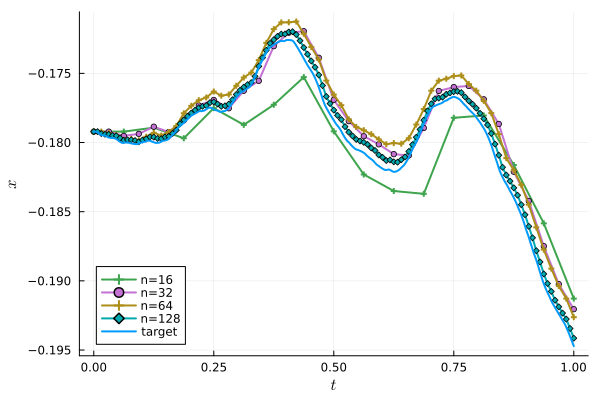
\includegraphics[scale=0.6]{img/approximation_linearhomogenous.png}
    \caption{Euler approximation of a sample solution of $\mathrm{d}X_t/\mathrm{d}t = W_t X_t$ with $X_0 \sim \mathcal{N}(0, 1)$, with a few mesh resolutions and with the target resolution.}
    \label{samplepathslinearhomogeneousrode}
\end{figure}

For a normal variable $N \sim \mathcal{N}(\mu, \sigma)$, the expectation of the random variable $e^N$ is $\mathbb{E}[e^N] = e^{\mu + \sigma^2/2}$. Hence,
\begin{equation}
    \mathbb{E}[e^{Z_i}] = e^{((t_{i+1}- t_i)^3)/24}.
\end{equation}
This is the contribution of this random variable to the mean of the exact solution. But we actually draw directly $Z_i$ and use $e^{\sum_i Z_i}$.

\begin{table}
    \begin{tabular}[htb]{|r|l|l|l|}
        \hline N & dt & error & std err \\
        \hline \hline
        16 & 0.0625 & 0.0379 & 0.0042 \\
        32 & 0.0312 & 0.0192 & 0.00208 \\
        64 & 0.0156 & 0.0095 & 0.00103 \\
        128 & 0.00781 & 0.00478 & 0.000519 \\
        256 & 0.00391 & 0.0024 & 0.000269 \\
        512 & 0.00195 & 0.00123 & 0.000143 \\
        1024 & 0.000977 & 0.000633 & 7.43e-5 \\
        2048 & 0.000488 & 0.000324 & 3.74e-5 \\
        4096 & 0.000244 & 0.000154 & 1.65e-5 \\
        8192 & 0.000122 & 7.71e-5 & 8.35e-6 \\
        16384 & 6.1e-5 & 3.76e-5 & 4.06e-6 \\
        \hline
    \end{tabular}
    \bigskip

    \caption{Mesh points (N), time steps (dt), strong error (error), and standard error (std err) of the Euler method for $\mathrm{d}X_t/\mathrm{d}t = W_t X_t$ for each mesh resolution $N$, with initial condition $X_0 \sim \mathcal{N}(0, 1)$ and a standard Wiener process noise $\{W_t\}_t$, on the time interval $I = [0.0, 1.0]$, based on $M = 500$ sample paths for each fixed time step, with the target solution calculated with $65536$ points. The order of strong convergence is estimated to be $p = 0.993$, with the 95\% confidence interval $[0.9497, 1.0362]$.}
    \label{tablinearhomogeneousrode}
\end{table}

Hence, once an Euler approximation of \eqref{linearhomogeneousrode} is computed, along with realizations $\{W_{t_i}\}_{i=0}^N$ of a sample path of the noise, we consider an exact solution given by
\begin{equation}
    \label{Xtlinearhomogeneousrode}
    X_{t_j} = X_0 e^{\sum_{i = 0}^{j-1}\left(\frac{1}{2}\left(W_{t_i} + W_{t_{i+1}}\right)(t_{i+1} - t_i) + Z_i\right)},
\end{equation}
for realizations $Z_i$ drawn from a normal distributions given by \eqref{linearhomogeneousZidistribution}. \cref{samplepathslinearhomogeneousrode} shows an approximate solution and a few sample paths of exact solutions associated with the given realizations of the noise on the mesh points.

\begin{figure}[htb]
    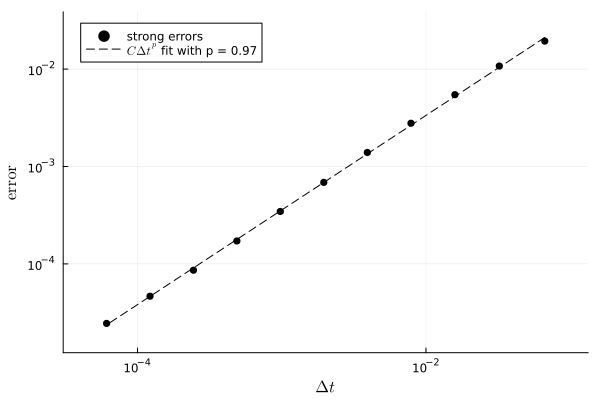
\includegraphics[scale=0.6]{img/order_wiener_linearhomogenous.png}
    \caption{Order of convergence $p = 0.974$ of the strong error of the Euler method for $\mathrm{d}X_t/\mathrm{d}t = W_t X_t$, based on \cref{tablinearhomogeneousrode}.}
    \label{figlinearhomogeneousrode}
\end{figure}

\cref{tablinearhomogeneousrode} shows the estimated strong error obtained from the $M = 200$ Monte Carlo simulations for each chosen time step $N_i = 2^4, \ldots, 2^{14}$, with initial condition $X_0 \sim \mathcal{N}(0, 1)$, on the time interval $[0, T] = [0.0, 1.0]$. The target resolution is set to $N_{\textrm{tgt}} = 2^{16}$, since we have the exact distribution for it. \cref{figlinearhomogeneousrode} illustrates the order of convergence.

\subsection{Non-homogeneous linear system of RODEs with different types of noises}

Next we consider a system of linear equations with a number of different types of noise. For most of these noises, the current knowledge expects a lower order of strong convergence than the strong order 1 we prove here. The aim of this section is to illustrate this improvement at once, for all such noises.

The system of equations takes the form
\begin{equation}
    \label{allnoisesRODEsystem}
    \begin{cases}
        \displaystyle \frac{\mathrm{d}\mathbf{X}_t}{\mathrm{d} t} = - \left\|\mathbf{Y}_t\right\|^2 \mathbf{X}_t + \mathbf{Y}_t, \qquad 0 \leq t \leq T, \\
        \left. \mathbf{X}_t \right|_{t = 0} = \mathbf{X}_0,
    \end{cases}
\end{equation}
where $\{\mathbf{X}_t\}_t$ is vector valued, and $\{\mathbf{Y}_t\}_t$ is a given vector-valued noise process with the same dimension as $\mathbf{X}_t$. Each coordinate of $\{\mathbf{Y}_t\}_t$ is a scalar noise process independent of the noises in the other coordinates. The scalar noises used in the simulations are the following, in the order of coordinates of $\mathbf{Y}_t$:
\begin{enumerate}
    \item A standard Wiener process;
    \item An Ornstein-Uhlenbeck process (OU) with drift $\nu = 0.3,$ diffusion $\sigma = 0.5,$ and initial condition $y_0 = 0.2$;
    \item A geometric Brownian motion process (gBm) with drift $\mu = 0.3,$ diffusion coefficient $\sigma = 0.5,$ and initial condition $y_0 = 0.2$;
    \item A non-autonomous homogeneous linear It\^o process (hlp) $\{H_t\}_t$ given by $\mathrm{d}H_t = (\mu_1 + \mu_2\sin(\vartheta t))H_t\;\mathrm{d}t + \sigma\sin(\vartheta t)H_t\;\mathrm{d}W_t$ with $\mu_1 = 0.5,$ $\mu_2 = 0.3,$ $\sigma = 0.5,$ $\vartheta=3\pi,$ and initial condition $H_0 = 0.2;$
    \item A compound Poisson process (cP) with rate $\lambda = 5.0$ and jump law following an exponential distribution with scale $\theta = 0.5;$
    \item A Poisson step process (sP) with rate $\lambda = 5.0$ and step law following a uniform distribution within the unit interval;
    \item An exponentially decaying Hawkes process with initial rate $\lambda_0 = 3.0$, base rate $a = 2.0$, exponential decay rate $\delta = 3.0$, and jump law following an exponential distribution with scale $\theta = 0.5;$
    \item A transport process of the form $t \mapsto \sum_{i=1}^{6} \sin^{1/3}(\omega_i t)$, where the frequencies $\omega_i$ are independent random variables following a Gamma distribution with shape parameter $\alpha = 7.5$ and scale $\theta = 2.0;$
    \item A fractional Brownian motion (fBm) process with Hurst parameter $H=0.6$ and initial condition $y_0 = 0.2$.
\end{enumerate}

\begin{table}
    \begin{tabular}[htb]{|r|l|l|l|}
        \hline N & dt & error & std err \\
        \hline \hline
        64 & 0.0156 & 0.196 & 0.0201 \\
        128 & 0.00781 & 0.0951 & 0.00972 \\
        256 & 0.00391 & 0.0473 & 0.00483 \\
        512 & 0.00195 & 0.0237 & 0.00242 \\
        \hline
    \end{tabular}
    \bigskip

    \caption{Mesh points (N), time steps (dt), strong error (error), and standard error (std err) of the Euler method for $\mathrm{d}\mathbf{X}_t/\mathrm{d}t = - \| \mathbf{Y}_t\|^2 \mathbf{X}_t + \mathbf{Y}_t$ for each mesh resolution $N$, with initial condition $\mathbf{X}_0 \sim \mathcal{N}(\mathbf{0}, \mathrm{I})$ and vector-valued noise $\{\mathbf{Y}_t\}_t$ with all the implemented noises, on the time interval $I = [0.0, 1.0]$, based on $M = 80$ sample paths for each fixed time step, with the target solution calculated with $262144$ points. The order of strong convergence is estimated to be $p = 1.017$, with the 95\% confidence interval $[0.8982, 1.1349]$.}
    \label{taballnoises}
\end{table}

\begin{figure}[htb]
    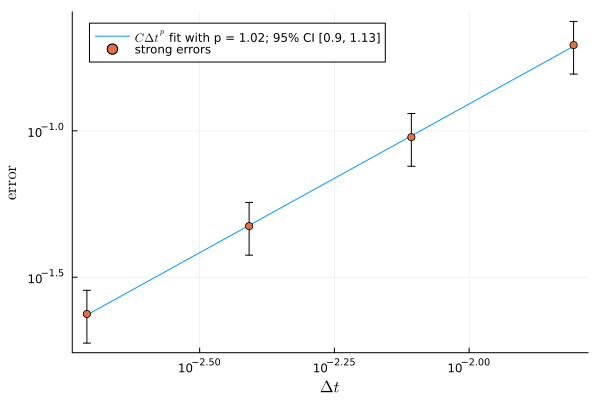
\includegraphics[scale=0.6]{img/order_allnoises.png}
    \caption{Order of convergence $p = 1.012$ of the strong error of the Euler method for $\mathrm{d}\mathbf{X}_t/\mathrm{d}t = - \left\|\mathbf{Y}_t\right\|^2 \mathbf{X}_t + \mathbf{Y}_t,$ based on \cref{taballnoises}.}
    \label{figallnoises}
\end{figure}

\cref{taballnoises} shows the estimated strong error obtained from the $M = 80$ Monte Carlo simulations for each chosen time step $N_i = 2^6, \ldots, 2^9$,  on the time interval $[0, T] = [0.0, 1.0]$. All coordinates of the initial condition are normally distributed with mean zero and variance 1. The target resolution is set to $N_{\textrm{tgt}} = 2^{18}$.

\cref{figallnoises} illustrates the obtained order of convergence, while \cref{figsamplepathsallnoises} illustrates some sample paths of all the noises used in this system.

\begin{figure}[htb]
    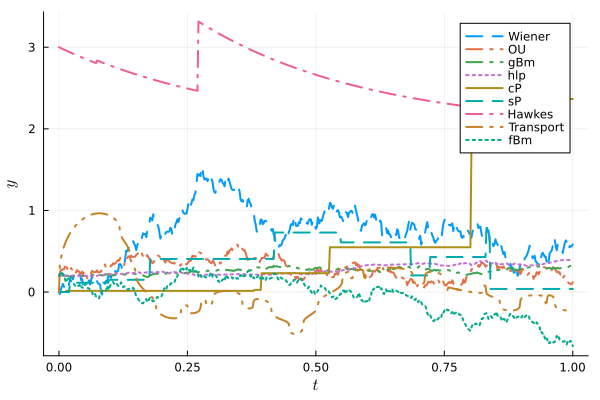
\includegraphics[scale=0.6]{img/noisepath_allnoises.png}
    \caption{Sample paths of all the noises used in the linear system \eqref{allnoisesRODEsystem}, mixing all different types of implemented noises.}
    \label{figsamplepathsallnoises}
\end{figure}

The strong order 1 convergence is not a suprise in the case of the Wiener and Ornstein-Uhlenbeck process since the corresponding RODE can be turned into an SDE with an additive noise. In this case, the Euler-Maruyama approximation for the noise part of the SDE is distributionally exact, and the Euler method for the RODE becomes equivalent to the Euler-Maruyama method for the SDE, and it is known that the Euler-Maruyama method for an SDE with additive noise is of strong order 1 \cite{HighamKloeden2021}. For the remaining noises, however, previous works would estimate the order of convergence to be below the order 1 attained here.

Notice we chose the hurst parameter of the fractional Brownian motion process to be between 1/2 and 1, so that the strong convergence is also of order 1, just like for the other types of noises in $\{\mathbf{Y}_t\}_t$. Previous knowledge would expect a strong convergence of order $H$, with $1/2 < H < 1,$ instead.

As for the geometric Brownian motion process, it is worth saying that its state at a given time $t$ depends solely on $t$ and on the state of an associated Wiener process at time $t$, so that the RODE can be transformed into another RODE with an additive noise. However, the corresponding nonlinear term does not have a global Lipschitz bound, so the strong order 1 does not follow from that. Our results, however, apply without further assumptions.

Finally, the homogeneous linear It\^o process is a multiplicative noise whose state at time $t$ cannot be written explicitly as a function of $t$ and $W_t.$ It requires the previous history $W_s$ of the associated Wiener process, for $0\leq s \leq t,$ hence the associated RODE cannot be transformed into a RODE with additive noise.

\subsection{Fractional Brownian motion noise}
\label{secfBmnoise}

Now, we consider again a linear equation, of the form
\begin{equation}
    \label{linearnonhomogeneousfbm}
    \begin{cases}
        \displaystyle \frac{\mathrm{d}X_t}{\mathrm{d} t} = -X_t + B^H_t, \qquad 0 \leq t \leq T, \\
        \left. X_t \right|_{t = 0} = X_0,
      \end{cases}
\end{equation}
except this time the noise $\{B^H_t\}_t$ is assumed to be a fractional Brownian motion (fBm) with Hurst parameter $0 < H < 1$. It turns out that, for $0 < H < 1/2$, the order of convergence is $H + 1/2$. The same seems to hold for a nonlinear dependency on the fBm, but the proof is more involved, depending on a fractional It\^o formula (see \cite[Theorem 4.2.6]{BHOB2008}, \cite[Theorem 4.1]{Bender2003}and \cite[Theorem 2.7.4]{Mishura2008}), based on the Wick It\^o Skorohod (WIS) integral (see \cite[Chapter 4]{BHOB2008}). A corresponding WIS isometry is also needed (see e.g. \cite[Theorem 4.5.6]{BHOB2008}), involving Malliavin calculus and fractional derivatives. For these reasons, we leave the nonlinear case to a subsequent work and focus on this simple linear example, which suffices to illustrate the peculiarity of the dependence on $H$ of the order of convergence. For this linear equation, the proof of convergence is done rigorously below, with the framework developed in the first sections.

We need to estimate the last term in \eqref{expectedestimateglobalerrorintegral} of \cref{propbasicestimate}, involving the steps of the term $f(t, x, y) = -x + y$, which in this case reduce to
\begin{equation}
    \label{stepfBm}
    f(s, X_{\tau^N(s)}^N, Y_s) - f(\tau^N(s), X_{\tau^N(s)}^N, Y_{\tau^N(s)}) = B^H_s - B^H_{\tau^N(s)},
\end{equation}
for $0 \leq s \leq T$. There are several ways to represent an fBm (see e.g. \cite{BHOB2008, Mishura2008}). We use the formula (see \cite[eq. (2.1)]{MandelbrotVanNess1968} or \cite[eq. (1.1)]{BHOB2008})
\begin{multline}
    \label{BHtintegralformula}
    B^H_t = \frac{1}{\Gamma(H + 1/2)}\left(\int_{-\infty}^0 \left( (t-s)^{H-1/2} - (-s)^{H-1/2}\right) \;\mathrm{d}W_s \right. \\
    \left. + \int_0^t (t - s)^{H-1/2} \;\mathrm{d}W_s\right),
\end{multline}
where $\Gamma(\cdot)$ is the well-known Gamma function. For the step, \eqref{BHtintegralformula} means that
\begin{multline}
    \label{BHtintegralformulastep}
    B^H_s - B^H_{\tau^N(s)} = \frac{1}{\Gamma(H + 1/2)}\left(\int_{-\infty}^{\tau^N(s)} \left( (s-\xi)^{H-1/2} - (\tau^N(s)-\xi)^{H-1/2}\right) \;\mathrm{d}W_\xi \right. \\
    \left. + \int_{\tau^N(s)}^s (s - \xi)^{H-1/2} \;\mathrm{d}W_\xi\right).
\end{multline}
Then, using the stochastic Fubini Theorem to exchange the order of integration (see, again, \cite[Section IV.6]{Protter2005}),
\begin{equation}
    \label{integralofstepfBm}
    \begin{aligned}
        \int_0^{t_j} & \left( f(s, X_{\tau^N(s)}^N, Y_s) - f(\tau^N(s), X_{\tau^N(s)}^N, Y_{\tau^N(s)}) \right)\;\mathrm{d}s \\
        & = \frac{1}{\Gamma(H + 1/2)}\int_0^{t_j} \int_{-\infty}^{\tau^N(s)} \left( (s-\xi)^{H-1/2} - (\tau^N(s)-\xi)^{H-1/2}\right) \;\mathrm{d}W_\xi \;\mathrm{d}s \\
        & \qquad + \frac{1}{\Gamma(H + 1/2)}\int_0^{t_j} \int_{\tau^N(s)}^s (s - \xi)^{H-1/2} \;\mathrm{d}W_\xi \;\mathrm{d}s \\
        & = \frac{1}{\Gamma(H + 1/2)}\int_{-\infty}^{0} \int_{0}^{t_j} \left( (s-\xi)^{H-1/2} - (\tau^N(s)-\xi)^{H-1/2}\right) \;\mathrm{d}s \;\mathrm{d}W_\xi \\
        & \qquad + \frac{1}{\Gamma(H + 1/2)}\int_{0}^{t_j} \int_{\tau^N(\xi)+\Delta t_N}^{t_j} \left( (s-\xi)^{H-1/2} - (\tau^N(s)-\xi)^{H-1/2}\right)  \;\mathrm{d}s \;\mathrm{d}W_\xi\\
        & \qquad + \frac{1}{\Gamma(H + 1/2)}\int_0^{t_j} \int_\xi^{\tau^N(\xi) + \Delta t_N} (s - \xi)^{H-1/2} \;\mathrm{d}s \;\mathrm{d}W_\xi. \\
    \end{aligned}
\end{equation}

For the first term, notice $\sigma \mapsto 1/(\sigma - \xi)^{H-1/2}$ is continuously differentiable on the interval $\sigma > \xi$, so that
\[
    (s-\xi)^{H-1/2} - (\tau^N(s)-\xi)^{H-1/2} = - (H-1/2)\int_{\tau^N(s)}^s (\sigma - \xi)^{H - 3/2} \;\mathrm{d}\sigma.
\]
Thus,
\[
    \int_{0}^{t_j} \left( (s-\xi)^{H-1/2} - (\tau^N(s)-\xi)^{H-1/2}\right) \;\mathrm{d}s = (H-1/2)\int_{0}^{t_j} \int_{\tau^N(s)}^s (\sigma - \xi)^{H - 3/2} \;\mathrm{d}\sigma \;\mathrm{d}s.
\]
Exchanging the order of integration yields
\begin{align*}
    \int_{0}^{t_j} \left( (s-\xi)^{H-1/2} \right. & \left. - (\tau^N(s)-\xi)^{H-1/2} \right) \;\mathrm{d}s \\
    & = (H-1/2)\int_{0}^{t_j} \int_{\sigma}^{\tau^N(\sigma) + \Delta t_N} (\sigma - \xi)^{H - 3/2} \;\mathrm{d}s \;\mathrm{d}\sigma \\
    & = (H-1/2)\int_{0}^{t_j} \left(\tau^N(\sigma) + \Delta t_N - \sigma\right) (\sigma - \xi)^{H - 3/2} \;\mathrm{d}\sigma.
\end{align*}
Hence,
\begin{multline*}
    \left|\int_{0}^{t_j} \left( (s-\xi)^{H-1/2} - (\tau^N(s)-\xi)^{H-1/2} \right) \;\mathrm{d}s\right| \\
    \leq (1/2 - H)\int_{0}^{t_j} \Delta t_N (\sigma - \xi)^{H - 3/2} \;\mathrm{d}\sigma.
\end{multline*}
Now, using the Lyapunov inequality and the It\^o isometry, and using the same trick as above,

\begin{align*}
    & \mathbb{E}\left[\left|\int_{-\infty}^{0} \int_{0}^{t_j} \left( (s-\xi)^{H-1/2} - (\tau^N(s)-\xi)^{H-1/2}\right) \;\mathrm{d}s \;\mathrm{d}W_\xi \right|\right] \\
    & \qquad\qquad \leq \left(\int_{-\infty}^{0} \left(\int_{0}^{t_j} \left( (s-\xi)^{H-1/2} - (\tau^N(s)-\xi)^{H-1/2}\right) \;\mathrm{d}s \right)^2 \;\mathrm{d}\xi \right)^{1/2} \\
    & \qquad\qquad \leq \Delta t_N \left(\int_{-\infty}^{0} \left( (1/2 - H)\int_0^{t_j} (\sigma - \xi)^{H-3/2} \;\mathrm{d}\sigma \right)^2 \;\mathrm{d}\xi \right)^{1/2} \\
    & \qquad\qquad \leq (1/2 - H)\Delta t_N \left(\int_{-\infty}^{0} \left(\int_0^T (\sigma - \xi)^{H-3/2} \;\mathrm{d}\sigma \right)^2 \;\mathrm{d}\xi \right)^{1/2}.
\end{align*}
Therefore,
\begin{multline}
    \label{firsttermfBm}
    \frac{1}{\Gamma(H + 1/2)}\Delta t_N \mathbb{E}\left[\left|\int_{-\infty}^{0} \int_{0}^{t_j} \left( (s-\xi)^{H-1/2} - (\tau^N(s)-\xi)^{H-1/2}\right) \;\mathrm{d}s \;\mathrm{d}W_\xi \right|\right] \\
    \leq c_H^{(1)}\Delta t_N,
\end{multline}
for a suitable constant $c_H^{(1)}$. We see this term is of order 1 in $\Delta t_N.$

The second term is similar,
\begin{align*}
    \int_{\tau^N(\xi)+\Delta t_N}^{t_j} & \left( (s-\xi)^{H-1/2} - (\tau^N(s)-\xi)^{H-1/2}\right) \;\mathrm{d}s \\ 
    & = (H-1/2)\int_{\tau^N(\xi)+\Delta t_N}^{t_j} \int_{\tau^N(s)}^s (\sigma - \xi)^{H - 3/2} \;\mathrm{d}\sigma \;\mathrm{d}s \\
    & = (H-1/2)\int_{\tau^N(\xi)+\Delta t_N}^{t_j} \int_\sigma^{\tau^N(\sigma) + \Delta t_N} (\sigma - \xi)^{H - 3/2} \;\mathrm{d}s \;\mathrm{d}\sigma \\
    & = (H-1/2)\int_{\tau^N(\xi)+\Delta t_N}^{t_j} \left(\tau^N(\sigma) + \Delta t_N - \sigma\right) (\sigma - \xi)^{H - 3/2} \;\mathrm{d}\sigma.
\end{align*}
Thus,
\begin{multline*}
    \left| \int_{\tau^N(\xi)+\Delta t_N}^{t_j} \left( (s-\xi)^{H-1/2} - (\tau^N(s)-\xi)^{H-1/2}\right) \;\mathrm{d}s \right| \\
    \leq (1/2 - H)\Delta t_N \int_{\tau^N(\xi)+\Delta t_N}^{t_j} (\sigma - \xi)^{H - 3/2} \;\mathrm{d}\sigma.
\end{multline*}
Hence,
\begin{align*}
    & \mathbb{E}\left[\left|\int_{0}^{t_j} \int_{\tau^N(\xi)+\Delta t_N}^{t_j} \left( (s-\xi)^{H-1/2} - (\tau^N(s)-\xi)^{H-1/2}\right) \;\mathrm{d}s \;\mathrm{d}W_\xi\right|\right] \\
    & \qquad\qquad \leq \left(\int_{0}^{t_j} \left(\int_{\tau^N(\xi)+\Delta t_N}^{t_j} \left( (s-\xi)^{H-1/2} - (\tau^N(s)-\xi)^{H-1/2}\right) \;\mathrm{d}s \right)^2 \;\mathrm{d}\xi \right)^{1/2} \\
    & \qquad\qquad \leq \Delta t_N (1/2 - H)\left(\int_{0}^{t_j} \left( \int_{\tau^N(\xi)+\Delta t_N}^{T} (\sigma - \xi)^{H-3/2} \;\mathrm{d}\sigma \right)^2 \;\mathrm{d}\xi \right)^{1/2}.
\end{align*}
Therefore,
\begin{multline}
    \label{secondtermfBm}
    \frac{1}{\Gamma(H + 1/2)}\mathbb{E}\left[\left|\int_{0}^{t_j} \int_{\tau^N(\xi)+\Delta t_N}^{t_j} \left( (s-\xi)^{H-1/2} - (\tau^N(s)-\xi)^{H-1/2}\right)  \;\mathrm{d}s \;\mathrm{d}W_\xi\right|\right] \\
    \leq c_H^{(2)}\Delta t_N,
\end{multline}
for a possibly different constant $c_H^{(2)}$. This term is also of order 1.

For the last term, we have
\begin{multline*}
    0 \leq \int_\xi^{\tau^N(\xi) + \Delta t_N} (s - \xi)^{H-1/2} \;\mathrm{d}s = \frac{1}{H + 1/2} (\tau^N(\xi) + \Delta t_N - \xi)^{H + 1/2} \\
    \leq \frac{1}{H + 1/2} \Delta t_N^{H + 1/2}.
\end{multline*}
so that, using the Lyapunov inequality and the It\^o isometry
\begin{multline*}
    \mathbb{E}\left[\left|\int_0^{t_j} \int_\xi^{\tau^N(\xi) + \Delta t_N} (s - \xi)^{H-1/2} \;\mathrm{d}s \;\mathrm{d}W_\xi\right|\right] \\
    \leq \left( \int_0^{t_j} \left(\int_\xi^{\tau^N(\xi) + \Delta t_N} (s - \xi)^{H-1/2} \;\mathrm{d}s\right)^2 \;\mathrm{d}\xi\right)^{1/2} \\ 
    \leq \left( \int_0^{t_j} \Delta t_N^{2H + 1} \;\mathrm{d}\xi\right)^{1/2} \leq t_j^{1/2} \Delta t_N^{H + 1/2}.
\end{multline*}
Therefore,
\begin{equation}
    \label{thirdtermfBm}
    \frac{1}{\Gamma(H + 1/2)}\mathbb{E}\left[\left|\int_0^{t_j} \int_\xi^{\tau^N(\xi) + \Delta t_N} (s - \xi)^{H-1/2} \;\mathrm{d}s \;\mathrm{d}W_\xi\right|\right] \leq c_H^{(3)} \Delta t_N^{H + 1/2},
\end{equation}
for a third constant $c_H^{(3)}$.

Putting the three estimates \eqref{firsttermfBm}, \eqref{secondtermfBm}, \eqref{thirdtermfBm} in \eqref{integralofstepfBm} we find that
\begin{multline}
    \mathbb{E}\left[\left|\int_0^{t_j} \left( f(s, X_{\tau^N(s)}^N, Y_s) - f(\tau^N(s), X_{\tau^N(s)}^N, Y_{\tau^N(s)}) \right)\;\mathrm{d}s\right|\right] \\
    \leq c_H^{(4)} \Delta t_N + c_H^{(3)} \Delta t_N^{H + 1/2},
\end{multline}
where $c_H^{(4)} = c_H^{(1)} + c_H^{(2)}$. Using this estimate in \cref{propbasicestimate} shows that the Euler method is of order $H + 1/2$, when $0 < H < 1/2$, and is of order 1, when $1/2 \leq H < 1$, having in mind that $H=1/2$ corresponds to the classical Wiener process.

In summary, we have proved the following result.
\begin{theorem}
    Consider the equation \eqref{linearnonhomogeneousfbm} where $\{B^H_t\}_t$ is a fractional Brownian motion (fBm) with Hurst parameter $0 < H < 1$. Suppose the initial condition $X_0$ satisfies
    \begin{equation}
        \label{EX0square2b}
        \mathbb{E}[|X_0|^2] < \infty.
    \end{equation}
    Then, the Euler scheme for this initial value problem is of strong order $H+1/2$, for $0 < H < 1/2$, and is of order $1$, for $1/2 \leq H < 1$. More precisely,
    \begin{equation}
        \max_{j=0, \ldots, N}\mathbb{E}\left[ \left| X_{t_j} - X_{t_j}^N \right| \right] \leq c_1 \Delta t_N + c_2 \Delta t_N^{H + 1/2}, \qquad \forall N \in \mathbb{N},
    \end{equation}
    for suitable constants $c_1, c_2 \geq 0$.
\end{theorem}

As for illustrating numerically the order of strong convergence, although the above linear equation has the explicit solution
\begin{equation}
    X_t = e^{-t}X_0 + \int_0^t e^{-(t-s)}B^H_s\;\mathrm{d}s,
\end{equation}
computing a distributionally exact solution of this form is a delicate process. Thus we check the convergence numerically by comparing the approximations with another Euler approximation on a much finer mesh.

More precisely, the Euler approximation is implemented for \eqref{linearnonhomogeneousfbm} with several values of $H$. We fix the time interval as $[0, T] = [0.0, 1.0]$, the initial condition as $X_0 \sim \mathcal{N}(0, 1),$ set the resolution for the target approximation to $N_{\textrm{tgt}} = 2^{18}$, choose the time steps for the convergence test as $\Delta t = 1/N$, with $N = 2^6, \ldots, 2^9,$ and use $M = 200$ samples for the Monte-Carlo estimate of the strong error. The fBm noise term is generated with the $\mathcal{O}(N)$ fast Fourier transform (FFT) method of Davies and Harte, as presented in \cite{DiekerMandjes2003} (see also \cite[Section 14.4]{HanKloeden2017}). \cref{taborderdepHfBm} shows the obtained convergence estimates, for a number of Hurst parameters, which is illustrated in \cref{figorderdepHfBm}, matching the theoretical estimate of $p = \min\{H+1/2, 1\}.$

\begin{table}
    \begin{tabular}[htb]{|c|c|c|c|}
        \hline $H$ & $p$ & $p_{\textrm{min}}$ & $p_{\textrm{max}}$ \\
        \hline \hline
        0.1 & 0.618829 & 0.558371 & 0.679264 \\
        0.2 & 0.714901 & 0.652603 & 0.777104 \\
        0.3 & 0.809808 & 0.751078 & 0.868671 \\
        0.4 & 0.882603 & 0.822044 & 0.942833 \\
        0.5 & 0.997408 & 0.93889 & 1.05586 \\
        0.7 & 1.00102 & 0.945619 & 1.05755 \\
        0.9 & 1.00198 & 0.936873 & 1.06707 \\
        \hline
    \end{tabular}
    \bigskip

    \caption{Hurst parameter $H$, order $p$ of strong convergence, and 95\% confidence interval $p_{\textrm{min}}$ and $p_{\textrm{max}}$, for a number of Hurst values.}
    \label{taborderdepHfBm}
\end{table}

\begin{figure}[htb]
    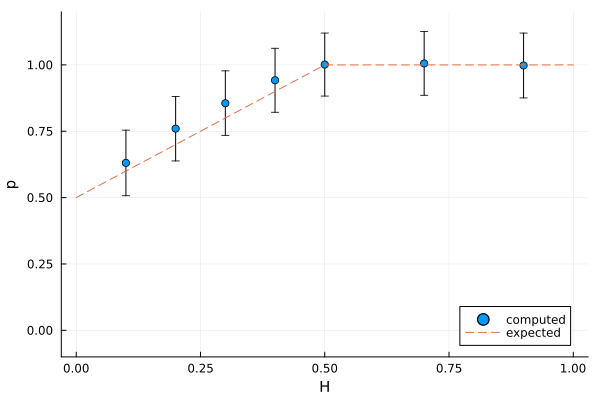
\includegraphics[scale=0.6]{img/order_dep_on_H_fBm.png}
    \caption{Order $p$ of strong convergence for each value of the Hurst parameter $H$ (scattered plot) along with the theoretical value $p=\min\{H + 1/2, 1\}$ (dashed line).}
    \label{figorderdepHfBm}
\end{figure}

\subsection{Population dynamics with harvest}
\label{secpopdyn}

Here, we consider a population dynamics problem modeled by a logistic equation with random coefficients, loosely inspired by \cite[Section 15.2]{HanKloeden2017}, with an extra term representing harvest:
\begin{equation}
    \label{rodepopulationdynamics}
    \frac{\mathrm{d}X_t}{\mathrm{d}t} = \Lambda_t X_t (1 - \frac{X_t}{r}) - \alpha H_t \frac{X_t}{r + X_t},
\end{equation}
where $r, \alpha > 0$ are constants and $\{\Lambda_t\}_{t \geq 0}$ and $\{H_t\}_{t \geq 0}$ are stochastic processes. The first term is a logistic growth, with carrying capacity $r$ and random specific growth $\Lambda_t$. The second term is the harvest term, with $\alpha$ being an overall modulation factor, the term $X_t / (r + X_t)$ accounting for the scarcity of the population when $X_t \ll r$, and with $0 \leq H_t \leq 1$ being a random harvest factor. 

More specifically, $\{\Lambda_t\}_{t \geq 0}$ is given by
\[
    \Lambda_t = \gamma (1 + \varepsilon \sin(G_t)),
\]
where $\gamma > 0,$ $0 < \varepsilon < 1,$ and $\{G_t\}_{t\geq 0}$ is a geometric Brownian motion (gBm) process, hence of the form \eqref{YtItonoise}-\eqref{Itonoiseterms}. A Wiener process is a natural choice, but we choose a gBm process instead since it is a multiplicative noise, thus the convergence would not be expected to be of strong order 1 based on previous works.

The harvest term $\{H_t\}_{t\geq 0}$ is a ``Poisson step'' process of the form
\[
    H_t = S_{N_t},
\]
where $\{N_t\}_{t\geq 0}$ is a Poisson point-process with rate $\lambda$, $S_0 = 0$, and the $S_i$, for $i=1, 2, \ldots$, are independent and identically distributed random variables with nonnegative values within the interval $[0, 1]$, independent also of the Poisson counter $\{N_t\}_{t\geq 0}$.

We suppose the initial condition is nonnegative and bounded almost surely, i.e.
\[
    0 \leq X_0 \leq R,
\]
for some $R > r$.

The noise process $\{\Lambda_t\}_{t \geq 0}$ itself satisfies
\[
    0 < \gamma - \varepsilon \leq \Lambda_t \leq \gamma + \varepsilon < 2\gamma, \qquad \forall t \geq 0.
\]

Define $f:\mathbb{R} \times \mathbb{R} \times \mathbb{R}^2 \rightarrow \mathbb{R}$ by
\[
    f(t, x, y) = \begin{cases}
        \displaystyle \gamma (1 + \varepsilon \sin(y_1)) x(r - x) - \alpha \frac{xy_2}{r + x}, & x \geq 0, \\
        0, & x < 0.
    \end{cases}
\]
The equation \eqref{rodepopulationdynamics} becomes
\[
    \frac{\mathrm{d}X_t}{\mathrm{d}t} = f(t, X_t, Y_t),
\]
where $\{Y_t\}_{t\geq 0}$ is the vector-valued process given in coordinates by $Y_t = (G_t, H_t)$.

Notice that $f(t, x, y) = 0$, for $x < 0$, for arbitrary $y=(y_1, y_2)$, while $f(t, x, y) < 0$, for $x \geq r$, $y_2 \geq 0$, and for arbitrary $y_1$. Since the noise $y_2 = H_t$ is always nonnegative, we see that the interval $0 \leq x \leq R$ is positively invariant and attracts the orbits with a nonnegative initial condition. Thus, the pathwise solutions of the initial-value problem under consideration are almost surely bounded as well.

The function $f=f(t, x, y)$ is continuously differentiable infinitely many times and with bounded derivatives within the positively invariant region. Hence, within the region of interest, all the conditions of \cref{thmsemimartingale} hold and the Euler method is of strong order 1.

Below, we simulate numerically the solutions of the above problem, with $\gamma = 0.8,$ $\varepsilon = 0.3,$ $r = 1.0,$ and $\alpha = \gamma r = 0.64$ The geometric Brownian motion process $\{G_t\}_{t\geq 0}$ is taken with drift coefficient $\mu = 1.0,$ diffusion coefficient $\sigma = 0.8,$ and initial condition $y_0 = 1.0.$ The Poisson process $\{N_t\}_{t \geq 0}$ is taken with rate $\lambda = 15.0$. And the step process $\{H_t\}_{t \geq 0}$ is taken with steps following a Beta distribution with shape parameters $\alpha = 5.0$ and $\beta = 7.0$. The initial condition $X_0$ is taken to be a Beta distribution with shape parameters $\alpha = 7.0$ and $\beta = 5.0$, hence we can take $R = 1$. We take $M = 200$ samples for the Monte-Carlo estimate of the strong error of convergence. For the target solution, we solve the equation with a time mesh with $N_{\mathrm{tgt}} = 2^{18}$, while for the approximations we take $N = 2^i$, for $i=4, \ldots, 9$.

Notice that we can write
\[
    \frac{\mathrm{d}X_t}{\mathrm{d}t} = \frac{X_t}{r + X_t} \left(r\Lambda_t - \alpha H_t - \frac{\Lambda_t}{r} X_t^2\right).
\]
Hence, when $\alpha H_t \geq r\Lambda_t$, the population decays for arbitrary $X_t > 0$, leading to an extinction of the population. The parameters chosen above keep the population from extinction but may often get close to the critical values.

\cref{tabpopdyn} shows the estimated strong error obtained for each mesh resolution, while \cref{figpopdyn} illustrates the order of convergence, estimated to be close enough to the theoretical value of strong order 1. Finally, \cref{figsamplepopdyn} shows an approximation sequence of a sample path.

\begin{table}
    \begin{tabular}[htb]{|r|l|l|l|}
        \hline N & dt & error & std err \\
        \hline \hline
        16 & 0.0625 & 0.00554 & 0.000253 \\
        32 & 0.0312 & 0.00269 & 0.000126 \\
        64 & 0.0156 & 0.00122 & 5.65e-5 \\
        128 & 0.00781 & 0.000637 & 2.87e-5 \\
        256 & 0.00391 & 0.000318 & 1.59e-5 \\
        512 & 0.00195 & 0.000169 & 8.22e-6 \\
        \hline
    \end{tabular}
    \bigskip

    \caption{Mesh points (N), time steps (dt), strong error (error), and standard error (std err) of the Euler method for population dynamics for each mesh resolution $N$, with initial condition $X_0 \sim \mathrm{Beta}(7.0, 5.0)$ and gBm and step process noises, on the time interval $I = [0.0, 1.0]$, based on $M = 200$ sample paths for each fixed time step, with the target solution calculated with $262144$ points. The order of strong convergence is estimated to be $p = 1.011$, with the 95\% confidence interval $[0.9759, 1.0453]$.}
    \label{tabpopdyn}
\end{table}

\begin{figure}[htb]
    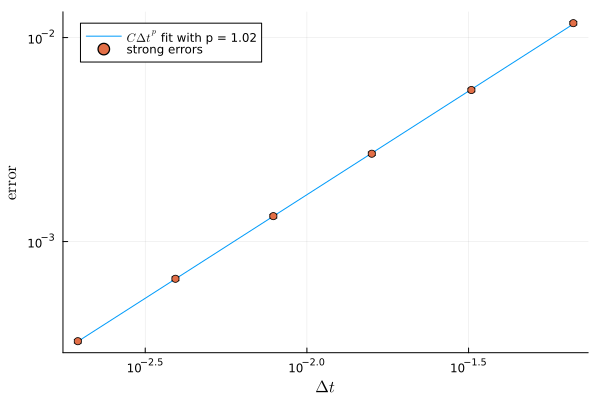
\includegraphics[scale=0.6]{img/order_popdyn_gBmPoisson.png}
    \caption{Order of convergence of the strong error of the Euler method for the population dynamics equation \eqref{rodepopulationdynamics}, based on \cref{tabpopdyn}.}
    \label{figpopdyn}
\end{figure}

\begin{figure}[htb]
    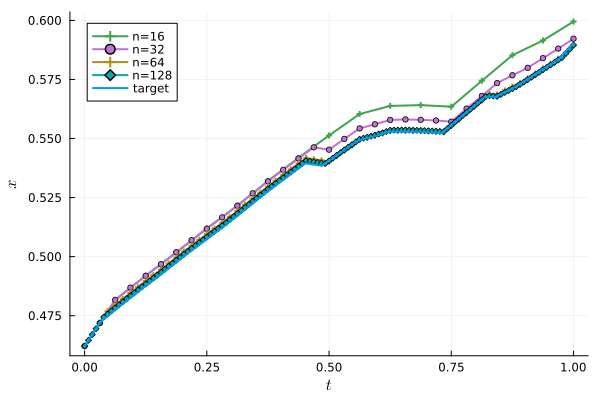
\includegraphics[scale=0.6]{img/sample_popdyn_gBmPoisson.png}
    \caption{An approximation sequence of a sample path solution of the population dynamics equation \eqref{rodepopulationdynamics}.}
    \label{figsamplepopdyn}
\end{figure}

\subsection{Mechanical structure under random Earthquake-like seismic disturbances}

Now we consider a simple mechanical structure model driven by a random disturbance in the form of a transport process, simulating seismic ground-motion excitations, inspired by the model in \cite{BogdanoffGoldbergBernard1961} (see also \cite[Chapter 18]{NeckelRupp2013} and \cite{HousnerJenning1964} with this and other models).

There are a number of models for earthquake-type forcing, such as the ubiquotous Kanai-Tajimi and the Clough-Penzien models, where the noise has a characteristic spectral density, determined by the mechanical properties of the ground layer. The ideia, from \cite{Kanai1957}, is that the spectrum of the noise at bedrock is characterized by a constant pattern, while at the ground surface it is modified by the vibration property of the ground layer. This interaction between the bedrock and the ground layer is modeled as a stochastic oscillator driven by a zero-mean Gaussian white noise, and whose solution leads to a noise with a characteristic power spectrum.

We follow, however, the Bogdanoff-Goldberg-Bernard model, which takes the form of a transport process noise. We chose the later so we can illustrate the improved convergence for such type of noise, complementing the other examples. The noise is described in more details shortly. Let us first introduce the model for the vibrations of the mechanical structure.

A single-storey building is considered, with its ground floor centered at position $M_t$ and its ceiling at position $M_t + X_t$. The random process $X_t$ refers to the motion relative to the ground. The ground motion $M_t$ affects the motion of the relative displacement $X_t$ as an excitation force proportional to the ground acceleration $\ddot M_t$. The damping and elastic forces are in effect within the structure. In this framework, the equation of motion for the relative displacement $X_t$ of the ceiling of the single-storey building takes the form

\begin{equation}
    \label{mechanicalstructuremodel}
    \ddot X_t + 2\zeta_0\omega_0\dot X_t + \omega_0^2 X_t = - \ddot M_t.
\end{equation}
where $\zeta_0$ and $\omega_0$ are damping and elastic model parameters depending on the structure of the building.

For the numerical simulations, the second-order equation is written as a system of first-order equations,
\[
    \begin{cases}
        \dot X_t = V_t, \\
        \dot V_t = - \omega_0^2 X_t - 2\zeta_0\omega_0 X_t - Y_t,
    \end{cases}
\]
where $\{V_t\}_t$ is the random velocity of the celing relative to the ground and where $\{Y_t\}_t$ is the stochastic noise excitation term given as the ground acceleration, $Y_t = \ddot M_t$, generated by an Earthquake and its aftershocks, or any other type of ground motion.

The structure is originally at rest, so we have the conditions
\[
    X_0 = 0, \quad V_0 = \dot X_0 = 0.
\]

In the Bogdanoff-Goldberg-Bernard model \cite{BogdanoffGoldbergBernard1961}, 
the excitation $\ddot M_t$ is made of a composition of oscillating signals with random frequencies, modulated by a linear attack rate followed by an exponential decay. This can be written, more precisely, as
\[
    \sum_{j=1}^n a_j t e^{-\delta_j t}\cos(\omega_j t + \theta_j).
\]

In order to simulate the start of the first shock-wave and the subsequent aftershocks, we modify this model sligthly to be a combination of such terms but at different incidence times. We also remove the attack rate from the excitation to obtain a rougher instantaneous, discontinuous excitation. This jump-like excitation is connected with a square power attack rate for the displacement itself. Finally, for simulation purposes, we model the displacement $M_t$ instead of modeling directly the excitation $\ddot M_t$, but in such a way that the ground-motion excitation follows essentially the proposed signal.

Thus, with this framework in mind, we model the ground displacement as a transport process composed of a series of time-translations of a square-power ``attack" front, with an exponentially decaying tail and an oscillating background wave:
\begin{equation}
    M_t = \sum_{i=1}^k \gamma_i (t - \tau_i)_+^2 e^{-\delta_i (t - \tau_i)}\cos(\omega_i (t - \tau_i)),
\end{equation}
where $k\in \mathbb{N}$ is given, $(t-\tau_i)_+ = \max\{0, t - \tau_i\}$ is the positive part of the function, and the parameters $\gamma_i,$ $\tau_i,$ $\delta_i,$ and $\omega_i$ are all random variables, with $\tau_i$ being exponentially distributed, and $\gamma_i$, $\delta_i$, and $\omega_i$ being uniformly distributed, each with different support values, and all of them independent of each other.

The excitation itself becomes
\begin{align*}
    \ddot M(t) = & 2\sum_{i=1}^k\gamma_i H(t - \tau_i) e^{-\delta_i (t - \tau_i)}\cos(\omega_i (t - \tau_i)) \\
        & + \sum_{i=1}^k\gamma_i (\delta_i^2 - \omega_i^2)(t - \tau_i)_+^2 e^{-\delta_i (t - \tau_i)}\cos(\omega_i (t - \tau_i)) \\
        & -2\sum_{i=1}^k\gamma_i (\delta_i + \omega_i) (t - \tau_i)_+ e^{-\delta_i (t - \tau_i)}\cos(\omega_i (t - \tau_i)) \\
        & +\delta_i\sum_{i=1}^k\omega_i\gamma_i (t - \tau_i)_+^2 e^{-\delta_i (t - \tau_i)}\sin(\omega_i (t - \tau_i)),
\end{align*}
where $H = H(s)$ is the Heaviside function, where, for definiteness, we set $H(s) = 1,$ for $s \geq 1,$ and $H(s) = 0$, for $s < 0$.

More specifically, for the numerical simulations, we use $\zeta_0 = 0.6$ and $\omega_0 = 15$ as the structural parameters. We set $T = 2.0,$ as the final time. For the transport process, we set $k=12$ and define the random parameters as the following exponential and uniform distributions: $\tau_i \sim \textrm{Exponential}(0.25),$ $\gamma_i \sim \textrm{Uniform}(0.0, 4.0),$ $\delta_i \sim \textrm{Uniform}(8.0, 12.0),$ and $\omega_i \sim \textrm{Uniform}(8\pi, 32\pi).$

For the mesh parameters, we set $N_{\textrm{tgt}} = 2^{18}$ and $N_i = 2^i$, for $i=6, \ldots, 9$. For the Monte-Carlo estimate of the strong error, we choose $M = 100.$ \cref{tableearthquake} shows the estimated strong error obtained with this setup, while \cref{figearthquake} illustrates the order of convergence. \cref{figearthquakenoise} shows a sample ground motion and the corresponding ground acceleration and its envelope.

\begin{table}
    \begin{tabular}[htb]{|r|l|l|l|}
        \hline N & dt & error & std err \\
        \hline \hline
        64 & 0.0312 & 2.09 & 0.18 \\
        128 & 0.0156 & 0.962 & 0.0761 \\
        256 & 0.00781 & 0.437 & 0.0356 \\
        512 & 0.00391 & 0.212 & 0.0175 \\
        \hline
    \end{tabular}
    \bigskip

    \caption{Mesh points (N), time steps (dt), strong error (error), and standard error (std err) of the Euler method for mechanical structure model under ground-shaking random excitations for each mesh resolution $N$, with initial condition $X_0 = \mathbf{0}$ and transport process noise, on the time interval $I = [0.0, 2.0]$, based on $M = 100$ sample paths for each fixed time step, with the target solution calculated with $262144$ points. The order of strong convergence is estimated to be $p = 1.106$, with the 95\% confidence interval $[1.0181, 1.1935]$.}
    \label{tableearthquake}
\end{table}

\begin{figure}[htb]
    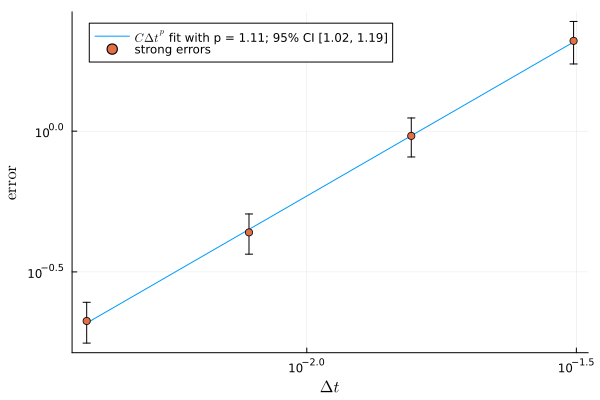
\includegraphics[scale=0.6]{img/convergence_earthquake.png}
    \caption{Order of convergence of the strong error of the Euler method for the mechanical structure model \eqref{mechanicalstructuremodel}, based on \cref{tableearthquake}.}
    \label{figearthquake}
\end{figure}

\begin{figure}[htb]
    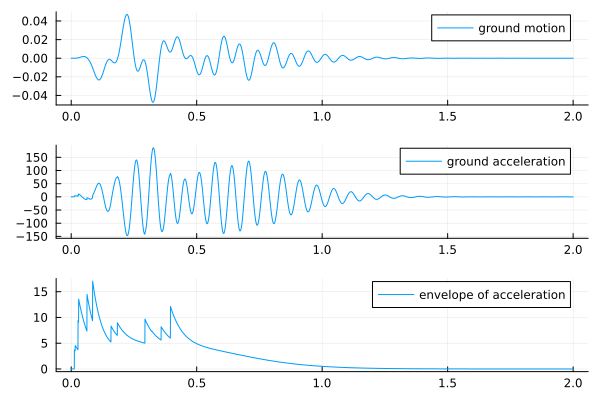
\includegraphics[scale=0.6]{img/noise_earthquake.png}
    \caption{Sample ground motion and the corresponding excitation (ground acceleration) and envelope of excitation (just the exponential decay, without the oscillations) for the mechanical structure model \eqref{mechanicalstructuremodel}.}
    \label{figearthquakenoise}
\end{figure}

\subsection{A toggle-switch model for gene expression}

Here, we consider the toggle-switch model in \cite[Section 7.8]{Asai2016}, originated from \cite{VerdCrombachJaeger2014}; see also \cite{StrasserTheisMarr2012}.

Toogle switches in gene expression consist of genes that mutually repress each other and exhibit two stable steady states of ON and OFF. It is a regulatory mechanism which is active during cell differentiation and is believed to act as a memory device, able to choose and maintain cell fate decisions.

We consider the following simple model as discussed in \cite[Section 7.8]{Asai2016}, of two interacting genes, $X$ and $Y$, with the concentration of their corresponding protein products at each time $t$ denoted by $X_t$ and $Y_t$. These are stochastic processes defined by the system of equations
\begin{equation}
    \label{toggleswitchsystem}
   \begin{cases}
   \frac{\displaystyle \mathrm{d}X_t}{\displaystyle \mathrm{d} t} = \left( A_t + \frac{\displaystyle X_t^4}{\displaystyle a^4 + X_t^4}\right)\left(\frac{\displaystyle b^4}{\displaystyle b^4 + Y_t^4}\right) - \mu X_t, \\
   \frac{\displaystyle \mathrm{d}Y_t}{\displaystyle \mathrm{d} t} = \left( B_t + \frac{\displaystyle Y_t^4}{\displaystyle c^4 + Y_t^4}\right)\left(\frac{\displaystyle d^4}{\displaystyle d^4 + X_t^4}\right) - \nu Y_t,
   \end{cases}
\end{equation}
on $t \geq 0$, with initial conditions $X_0$ and $Y_0$, where $\{A_t\}_{t\geq 0}$ and $\{B_t\}_{t\geq 0}$ are given stochastic process representing the external activation on each gene; $a$ and $c$ determine the auto-activation thresholds; $b$ and $d$ determine the thresholds for mutual repression; and $\mu$ and $\nu$ are protein decay rates. In this model, the external activations $A_t$ is taken to be a compound Poisson process, while $B_t$ is non-autonomous homogeneous linear It\^o process of the form $\mathrm{d}B_t = (\mu_1 + \mu_2\sin(\vartheta t))B_t\;\mathrm{d}t + \sigma\sin(\vartheta t)B_t\;\mathrm{d}W_t$.

In the simulations below, we use parameters similar to those in \cite[Section 7.8]{Asai2016}. We fix $a = c = 0.25$; $b = d = 0.4$; and $\mu = \nu = 0.75$. The initial conditions are set to $X_0 = Y_0 = 4.0$. The external activation $\{A_t\}$ is a compound Poisson process with Poisson rate $\lambda = 5.0$ and jumps uniformly distributed within $[0.0, 0.5]$, while $\{B_t\}_t$ is taken with $\mu_1 = 0.7,$ $\mu_2 = 0.3,$ $\sigma = 0.3,$ $\vartheta=3\pi,$ and initial condition $B_0 = 0.2;$. The convergence estimate is done over the interval $[0, 5.0]$, while some illustrative solutions are over a longer interval $[0, 10.0]$.

We do not have an explicit solution for the equation so we use as target for the convergence an approximate solution via Euler method at a much higher resolution.

For the mesh parameters, we set $N_{\textrm{tgt}} = 2^{18}$ and $N_i = 2^i$, for $i=5, \ldots, 9$. For the Monte-Carlo estimate of the strong error, we choose $M = 100.$ \cref{tabletoggleswitch} shows the estimated strong error obtained with this setup, while \cref{figtoggleswitch} illustrates the order of convergence. \cref{figtoggleswitchevolution} shows a sample solution, while \cref{figtoggleswitchnoise} illustrates the two components $(A_t, B_t)$ of a sample noise.

\begin{table}
    \begin{tabular}[htb]{|r|l|l|l|}
        \hline N & dt & error & std err \\
        \hline \hline
        32 & 0.156 & 0.623 & 0.0354 \\
        64 & 0.0781 & 0.3 & 0.0169 \\
        128 & 0.0391 & 0.146 & 0.00818 \\
        256 & 0.0195 & 0.0716 & 0.00403 \\
        512 & 0.00977 & 0.0354 & 0.00202 \\
        \hline
    \end{tabular}
    \bigskip

    \caption{Mesh points (N), time steps (dt), strong error (error), and standard error (std err) of the Euler method for a toggle-switch model of gene regulation for each mesh resolution $N$, with initial condition $X_0 = 4.0, Y_0 = 4.0$ and coupled compound Poisson process and geometric Brownian motion noises, on the time interval $I = [0.0, 5.0]$, based on $M = 100$ sample paths for each fixed time step, with the target solution calculated with $262144$ points. The order of strong convergence is estimated to be $p = 1.034$, with the 95\% confidence interval $[0.9865, 1.0809]$.}
    \label{tabletoggleswitch}
\end{table}

\begin{figure}[htb]
    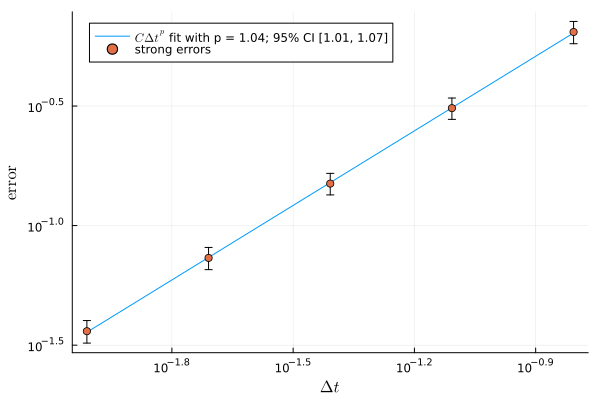
\includegraphics[scale=0.6]{img/order_toggleswitch.png}
    \caption{Order of convergence of the strong error of the Euler method for the toggle-switch model \eqref{toggleswitchsystem}, based on \cref{tabletoggleswitch}.}
    \label{figtoggleswitch}
\end{figure}

\begin{figure}[htb]
    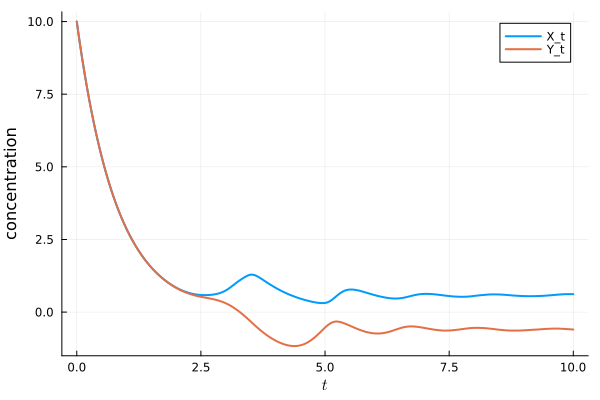
\includegraphics[scale=0.6]{img/evolution_toggleswitch.png}
    \caption{Evolution of a sample solution of the toggle-switch model \eqref{toggleswitchsystem}.}
    \label{figtoggleswitchevolution}
\end{figure}

\begin{figure}[htb]
    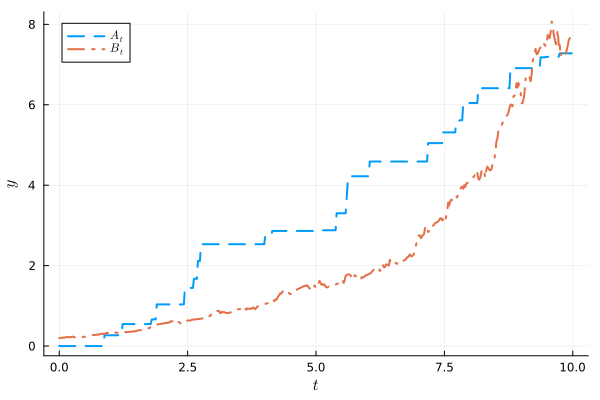
\includegraphics[scale=0.6]{img/noises_toggleswitch.png}
    \caption{Noise sample paths for the toggle-switch model \eqref{toggleswitchsystem}.}
    \label{figtoggleswitchnoise}
\end{figure}

\subsection{An actuarial risk model}

A classical model for the surplus $U_t$ at time $t$ of an insurance company is the Cram\'er-Lundberg model (see e.g. \cite{GerberShiu1998}) given by
\[
  U_t = U_0 + \gamma t - \sum_{i=1}^{N_t} C_i,
\]
where $U_0$ is the initial capital, $\gamma$ is a constant premium rate received from the insurees, $C_i$ is a random variable representing the value of the $i$-th claim paid to a given insuree, and $N_t$ is the number of claims up to time $t$. The process $\{N_t\}_t$ is modeled as a Poisson counter, so that the accumulated claims form a compound Poisson process. It is also common to use inhomogeneous Poisson processes and Hawkes self-exciting process, or combinations of such processes for the incidence of the claim, but the classical model uses a homogeneous Poisson counter.

The model above, however, does not take into account the variability of the premium rate received by the company, nor the investiment of the accumulated reserves, among other things. Several diffusion type models have been proposed to account for these and other factors. We consider here a simple model, with a randomly perturbed premium and with variable rentability.

More precisely, we start by rewriting the above expression as the following jump (or impulse) differential equation
\[
  \mathrm{d}U_t = \gamma\;\mathrm{d}t - \mathrm{d}C_t,
\]
where
\[
  C_t = \sum_{i=1}^{N_t} C_i.
\]

The addition of an interest rate $r$ leads to
\[
  \mathrm{d}U_t = r U_t \mathrm{d}t + \gamma\;\mathrm{d}t - \mathrm{d}C_t.
\]

Assuming a premium rate perturbed by a white noise and assuming the interest rate as a process $\{R_t\}_t$, we find
\[
  \mathrm{d}U_t = R_t U_t\;\mathrm{d}t + \gamma\;\mathrm{d}t + \varepsilon\;\mathrm{d}W_t - \mathrm{d}C_t,
\]
so the equation becomes
\[
  \mathrm{d}U_t = (\gamma + R_t U_t)\;\mathrm{d}t + \varepsilon\;\mathrm{d}W_t - \mathrm{d}C_t.
\]

Since we can compute exactly the accumulated claims $C_t$, we subtract it from $U_t$ to get rid of the jump term. We also subtract an Ornstein-Uhlenbeck process, in the classical way to transform an SDE into a RODE. So, defining
\[
  X_t = U_t - C_t - O_t,
\]
where $\{O_t\}_t$ is given by
\[
  \mathrm{d}O_t = -\nu O_t\;\mathrm{d}t + \varepsilon\;\mathrm{d}W_t,
\]
we obtain
\[
  \mathrm{d}X_t = (\gamma + R_t U_t)\;\mathrm{d}t + \nu O_t\;\mathrm{d}t = (\gamma + R_t (X_t + C_t + O_t))\;\mathrm{d}t + \nu O_t\;\mathrm{d}t.
\]

This leads us to the linear random ordinary differential equation
\begin{equation}
    \label{riskmodel}
    \frac{\mathrm{d}X_t}{\mathrm{d}t} = R_t X_t + R_t (C_t + O_t) + \nu O_t + \gamma.
\end{equation}

This equation has the explicit solution
\[
  X_t = X_0 e^{\int_0^t R_s\;\mathrm{d}s} + \int_0^t e^{\int_s^t R_\tau\;\mathrm{d}\tau} (R_s (C_s + O_s) + \nu O_s + \gamma)\;\mathrm{d}s.
\]

As for the interest rate process $\{R_t\}_t$, there is a vast literature with models for it, see e.g. \cite[Chapter 3]{BrigoMercurio2006} in particular Table 3.1. Here, we consider the Dothan model (\cite[Section 3.2.2]{BrigoMercurio2006} of the aforementioned reference), which consists simply of a geometric Brownian motion process
\[
  \mathrm{d}R_t = \mu R_t \;\mathrm{d}t + \sigma R_t\;\mathrm{d}t,
\]
with $R_t = r_0$, where $\mu, \sigma, r_0$ are positive constants. This has an explicit solution
\[
  R_t = r_0 e^{(\mu - \sigma^2/2)t + \sigma W_t},
\]
so that the equation \eqref{riskmodel} for $\{X_t\}_t$ is a genuine random ODE.

Once the solution of $\{X_t\}_t$ is obtained, we find an explicit formula for the surplus $U_t = X_t + C_t + O_t$, namely
\[
  U_t = C_t + O_t + X_0 e^{\int_0^t R_s\;\mathrm{d}s} + \int_0^t e^{\int_s^t R_\tau\;\mathrm{d}\tau} (R_s (C_s + O_s) + \nu O_s + \gamma)\;\mathrm{d}s,
\]
with $\{R_t\}_t$ as above.

For the numerical simulations, we use $O_0 = 0$, $\nu = 5$ and $\varepsilon = 0.8$, for the Ornstein-Uhlenbeck process $\{O_t\}_t$; $\lambda = 8.0$ and $C_i \sim \mathrm{Uniform}(0, 0.2)$, for the compound Poisson process $\{C_t\}$; $R_0 = 0.2$, $\mu = 0.02$ and $\sigma = 0.4$, for the interest rate process $\{R_t\}_t$; and we take $X_0 = 1.0$, so that $U_0 = X_0 + O_0 + R_0 = 1.2$. We set $T = 3.0,$ as the final time.

For the mesh parameters, we set $N_{\textrm{tgt}} = 2^{18}$ and $N_i = 2^i$, for $i=6, \ldots, 9$. For the Monte-Carlo estimate of the strong error, we choose $M = 400.$ \cref{tableriskmodel} shows the estimated strong error obtained with this setup, while \cref{figriskmodel} illustrates the order of convergence. \cref{figriskmodelnoise} shows a sample path of the noise, which is composed of three processes, while \cref{figriskmodelsurplus} shows a sample path of the surplus.

\begin{table}
    \begin{tabular}[htb]{|r|l|l|l|}
        \hline N & dt & error & std err \\
        \hline \hline
        64 & 0.0469 & 0.223 & 0.0167 \\
        128 & 0.0234 & 0.115 & 0.00878 \\
        256 & 0.0117 & 0.0579 & 0.00405 \\
        512 & 0.00586 & 0.0286 & 0.00209 \\
        \hline
    \end{tabular}
    \bigskip

    \caption{Mesh points (N), time steps (dt), strong error (error), and standard error (std err) of the Euler method for a risk model for each mesh resolution $N$, with initial condition $X_0 = 1.0$ and coupled Ornstein-Uhlenbeck, geometric Brownian motion, and compound Poisson processes, on the time interval $I = [0.0, 3.0]$, based on $M = 400$ sample paths for each fixed time step, with the target solution calculated with $262144$ points. The order of strong convergence is estimated to be $p = 0.987$, with the 95\% confidence interval $[0.9019, 1.0727]$.}
    \label{tableriskmodel}
\end{table}

\begin{figure}[htb]
    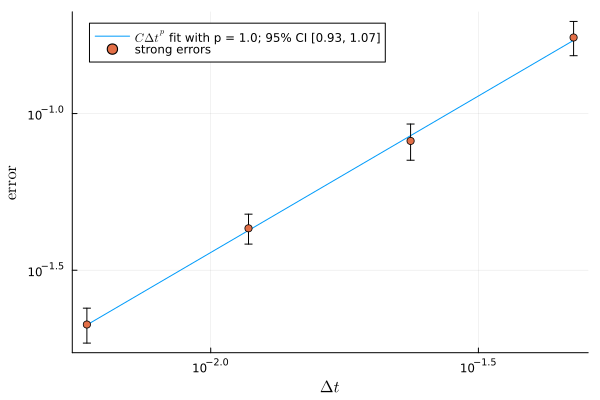
\includegraphics[scale=0.6]{img/convergence_riskmodel.png}
    \caption{Order of convergence of the strong error of the Euler method for the actuarial risk model \eqref{riskmodel}, based on \cref{tableriskmodel}.}
    \label{figriskmodel}
\end{figure}

\begin{figure}[htb]
    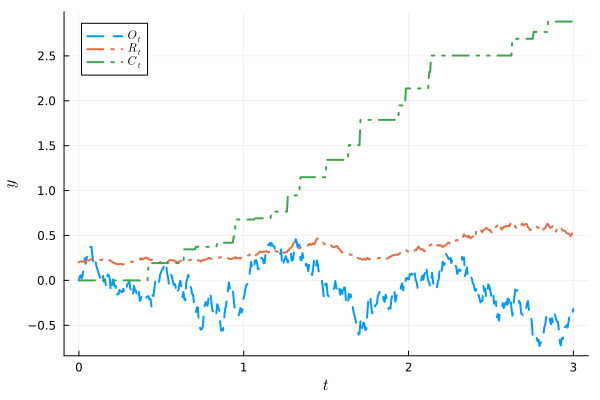
\includegraphics[scale=0.6]{img/riskmodel_noises.png}
    \caption{Sample noises for the risk model \eqref{riskmodel}.}
    \label{figriskmodelnoise}
\end{figure}

\begin{figure}[htb]
    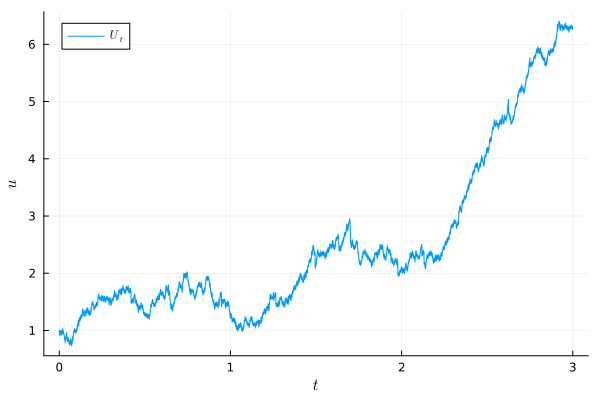
\includegraphics[scale=0.6]{img/riskmodel_surplus.png}
    \caption{Sample surplus solution for the risk model \eqref{riskmodel}.}
    \label{figriskmodelsurplus}
\end{figure}

\subsection{A random Fisher-KPP nonlinear PDE driven by boundary noise}

Finally, we simulate a Fisher-KPP equation with random boundary conditions, as inspired by the works of \cite{SalakoShen2020}  and \cite{FreidlinWentzell1992}. The first work addresses the Fisher-KPP equation with a random reaction coefficient, while the second work considers more general reaction-diffusion equations but driven by random boundary conditions.

The intent here is to illustrate the strong order 1 convergence rate on a discretization of a nonlinear partial differential equation. We use the method of lines (MOL), with finite differences in space, to approximate the random partial differential equation (PDE) by a system of random ODEs.

The deterministic Fisher-KPP equation is a nonlinear parabolic equation of reaction-diffusion type, with origins in \cite{Fisher1937} and \cite{KPP1937}. It models inhomogeneous population growth and many other phenomena displaying wave propagation, such as combustion front wave propagation, physiollogy, crystallography pattern formation, and so on.

We consider the Fisher-KPP equation driven by Neumann boundary conditions, with a random influx on the left end point and no flux on the right end point.

The equation takes the form
\begin{equation}
    \label{fisherkpprode}
    \frac{\partial u}{\displaystyle \partial t} = \mu\frac{\partial^2 u}{\partial x^2} + \lambda u\left(1 - \frac{u}{u_m}\right), \quad (t, x) \in (0, \infty) \times (0, 1),
\end{equation}
endowed with the boundary conditions
\begin{equation}
    \label{fisherkppbc}
    \frac{\partial u}{\partial x}(t, 0) = - Y_t, \quad \frac{\partial u}{\partial x}(t, 1) = 0,
\end{equation}
and a given a initial condition
\[
   u(0, x) = u_0(x).
\]

The unknown $u(t, x)$ represents the density of a given quantity at time $t$ and point $x$; $D$ is a diffusivity coefficient; $\lambda$ is a reaction, or proliferation, coefficient; and $u_m$ is a carrying capacity density coefficient.

The random process $\{Y_t\}_t$, which drives the flux on the left boundary point, is taken to be a colored noise modulated by an exponentially decaying Hawkes process, representing random wave trains of incoming populations. More precisely, $Y_t = H_t O_t$, where $\{H_t\}_t$ is a Hawkes process with initial rate $\lambda_0 = 3.0$, base rate $a = 0.3$, exponential decay rate $\delta = 5.0$, and jump law following an exponential distribution with scale $\theta = 1/1.8;$ and $\{O_t\}_t$ is an Orstein-Uhlenbeck process with $O_0 = 0.0,$ time-scale $\tau = 0.005$, drift $\nu = 1/\tau$ and diffusion $\sigma = \tilde \sigma/\tau,$ where $\tilde\sigma = 0.1.$

This equation displays traveling wave solutions with a minimum wave speed of $2 \sqrt{\lambda \mu}$. We choose $\lambda = 10$ and $\mu= 0.009$, so the limit traveling speed is about $0.6$. The carrying capacity is set to $u_m = 1.0$.

The initial condition is taken to be zero, $u_0(x) = 0$, so all the population originates from the left boundary influx.

The mass within the region $0\leq x \leq 1$ satisfies
\[
   \frac{\mathrm{d}}{\mathrm{d} t} \int_0^1 u(t, x) \;\mathrm{d}x = \mu\int_0^1 u_{xx}(t, x) \;\mathrm{d}x + \lambda \int_0^1 u(t, x)\left(1 - \frac{u(t, x)}{u_m}\right)\;\mathrm{d}x.
\]
Using the boundary conditions, we find that
\[
   \frac{\mathrm{d}}{\mathrm{d}t} \int_0^1 u(t, x) \;\mathrm{d}x = \mu Y_t  + \frac{\lambda}{u_m} \int_0^1 u(t, x)\left(u_m - u(t, x)\right)\;\mathrm{d}x,
\]
which is nonnegative, provided $0 \leq u \leq u_m$ and $Y_t \geq 0$.

The equation involves a nonlinear term which is not globally Lipschitz continuous, but, similiarly to the population dynamics model considered in \cref{secpopdyn}, the region $0 \leq u(t, x) \leq u_m$ is invariant, so that the nonlinear term can be modified outside this region in order to satisfy the required uniform global estimates without affecting the dynamics within this region. The initial condition is chosen to be within this region almost surely. The procedure is the same as that done in \cref{secpopdyn}, so the details are omited.

For the time-mesh parameters, we set $N_{\textrm{tgt}} = 2^{18}$ and $N_i = 2^5, 2^7, 2^9.$ The spatial discretization is done with finite differences, with the number of spatial points depending on the time mesh, for stability and convergence reasons. Indeed, the Von Neumann stability analysis requires that $2\mu\Delta t / \Delta_x^2 \leq 1.$ With that in mind, for each $N_i = 2^5, 2^7, 2^9$, we take the $K_i + 1$ spatial points $0 = x_0 < \ldots x_{K_i},$ with $K_i = 2^3,$ $2^4,$ and $2^5,$ respectively, while for the target solution, we use $K_{\textrm{tgt}} = 2^9.$

For the Monte-Carlo estimate of the strong error, we choose $M = 40.$ \cref{tablefisherkpp} shows the estimated strong error obtained with this setup, while \cref{figfisherkpp} illustrates the order of convergence.

\begin{table}
    \begin{tabular}[htb]{|r|l|l|l|}
        \hline N & dt & error & std err \\
        \hline \hline
        32 & 0.0625 & 128.0 & 20.4 \\
        128 & 0.0156 & 30.2 & 4.82 \\
        512 & 0.00391 & 6.53 & 1.04 \\
        \hline
    \end{tabular}
    \bigskip

    \caption{Mesh points (N), time steps (dt), strong error (error), and standard error (std err) of the Euler method for the Fisher-KPP equation for each mesh resolution $N$, with initial condition $X_0 = 0$ and Hawkes-modulated Ornstein-Uhlenbeck colored noise, on the time interval $I = [0.0, 2.0]$, based on $M = 40$ sample paths for each fixed time step, with the target solution calculated with $262144$ points. The order of strong convergence is estimated to be $p = 1.072$, with the 95\% confidence interval $[0.9558, 1.1882]$.}
    \label{tablefisherkpp}
\end{table}

\begin{figure}[htb]
    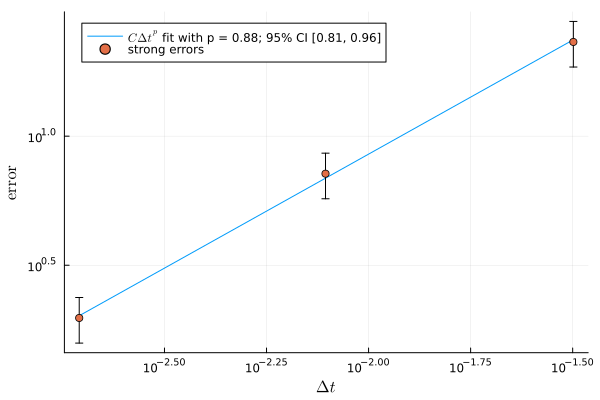
\includegraphics[scale=0.6]{img/order_fisherkpp.png}
    \caption{Order of convergence of the strong error of the Euler method for the Fisher-KPP model \eqref{fisherkpprode}-\eqref{fisherkppbc}, based on \cref{tablefisherkpp}.}
    \label{figfisherkpp}
\end{figure}

\begin{thebibliography}{25}
    \bibitem{Asai2016} Y. Asai, \emph{Numerical Methods for Random Ordinary Differential Equations and their Appli-
    cations in Biology and Medicine.} Dissertation, Institut f\"ur Mathematik, Goethe Universit\"at Frankfurt am Main, 2016.

    \bibitem{AsaiKloeden2016} Y. Asai, P. E. Kloeden, Numerical schemes for random ODES with affine noise, \emph{Numer. Algorithms} 72 (2016), 155--171.

    \bibitem{Bender2003} C. Bender, An It\^o formula for generalized functionals of a fractional Brownian motion with arbitrary Hurst parameter, \emph{Stochastic Processes and their Applications,} 104 (2003), 81--106.

    \bibitem{Julia2017} J. Bezanson, A. Edelman, S. Karpinski, and V. B. Shah, Julia: A fresh approach to numerical computing, \emph{Siam Review,} 59 (2017), no. 1, 65--98.

    \bibitem{BHOB2008} F. Biagini, Y. Hu, B. {\O}ksendal, and T. Zhang. \emph{Stochastic Calculus for Fractional Brownian Motion and Applications,} Springer-Verlag, London, 2008.

    \bibitem{BogdanoffGoldbergBernard1961} J. L. Bogdanoff, J. E. Goldberg, and M. C. Bernard, Response of a simple structure to a random earthquake-type disturbance, \emph{Bulletin of the Seismological Society of America,} 51 (1961), no. 2, 293--310.

    \bibitem{BrigoMercurio2006}, D. Brigo, F. Mercurio, \emph{Interest Rate Models - Theory and Practice,} Springer-Verlag, Berlin, Heidelberg, 2006.

    \bibitem{Clark1987} D. S. Clark, Short proof of a discrete Gronwall inequality, \emph{Discrete Applied Mathematics,} Vol. 16 (1987) no. 3, 279--281.

    \bibitem{CoddingtonLevinson1985} E. A. Coddington and N. Levinson, \emph{Theory of Ordinary Differential Equations,} New York: McGraw-Hill, 1987.

    \bibitem{DiekerMandjes2003} A. B. Dieker and M. Mandjes, On spectral simulation of fractional Brownian motion, \emph{Probability in the Engineering and Informational Sciences,} 17 (2003), 417--434.

    \bibitem{Fisher1937} R. A. Fisher, The wave of advance of advantageous genes, \emph{Annals of Eugenics,} 7 (1937), no. 4, 355--369.

    \bibitem{FreidlinWentzell1992} M. I. Freidlin and A. D. Wentzell, Reaction-diffusion equations with randomly perturbed boundary conditions, \emph{Ann. Probab.} 20 (1992), no. 2, 963--986.

    \bibitem{GerberShiu1998} H. U. Gerber, E. S. W. Shiu, On the time value of ruin, North American Actuarial J. 
    vol. 2 (1998), no. 1, 48--72.

    \bibitem{GHLOUZ1993} H. Gjessing, H. Holden, T. Lindstr{\o}n, B. {\O}ksendal, J. Ub{\o}e, and T.-S. Zhang, The Wick product, \emph{Vol. 1 Proceedings of the Third Finnish-Soviet Symposium on Probability Theory and Mathematical Statistics,} Turku, Finland, August 13--16, 1991, edited by H. Niemi, G. H\"ognas, A. N. Shiryaev and A. V. Melnikov, Berlin, Boston: De Gruyter, 1993, pp. 29-67.

    \bibitem{GiraultRaviart1981} V. Girault and P.-A. Raviart, \emph{Finite-Element Approximation of the Navier-Stokes Equations,} Lecture Notes in Mathematics, vol. 749, Springer-Verlag, Berlin, Heidelberg, 1981.

    \bibitem{Gronwall1919} T. H. Gronwall, Note on the derivatives with respect to a parameter of the solutions of a system of differential equations, \emph{Ann. of Math.} (2) 20 (1919), 292--296.

    \bibitem{GruneKloeden2001} L. Gr\"une and P.E. Kloeden, Higher order numerical schemes for affinely controlled nonlinear systems, \emph{Numer. Math.} 89 (2001), 669--690.

    \bibitem{HanKloeden2017} X. Han and P. E. Kloeden, \emph{Random Ordinary Differential Equations and Their Numerical Solution,} Probability Theory and Stochastic Modelling, vol. 85, Springer Singapore, 2017.

    \bibitem{HighamKloeden2021} D. J. Higham and P. E. Kloeden, \emph{An Introduction to the Numerical Simulation of Stochastic Differential Equations,} Volume 169 of Other Titles in Applied Mathematics, SIAM, 2021.

    \bibitem{HousnerJenning1964} G. W. Housner and Paul C. Jennings, Generation of artificial Earthquakes, Journal of the Engineering Mechanics Division, 90 (1964), no. 1.

    \bibitem{JentzenKloeden2011} A. Jentzen and P.E. Kloeden, \emph{Taylor Approximations of Stochastic Partial Differential Equations,} CBMS Lecture series, SIAM, Philadelphia, 2011.

    \bibitem{JentzenKloedenNeuenkirch2009} A. Jentzen, P.E. Kloeden, and A. Neuenkirch, Pathwise approximation of stochastic differential equations on domains: Higher order convergence rates without global Lipschitz coefficients, \emph{Numer. Math.} 112 (2009), no. 1, 41--64.

    \bibitem{Kanai1957} K. Kanai, Semi-empirical formula for the seismic characteristics of the ground, \emph{Bull. Earthq. Res. Inst.,} Vol. 35 (1957), University of Tokyo.

    \bibitem{KloedenJentzen2007} A. Jentzen, P.E. Kloeden,, Pathwise convergent higher order numerical schemes for random ordinary differential equations, \emph{Proc. R. Soc. A} 463 (2007), 2929--2944.

    \bibitem{KPP1937} A. N. Kolmogorov, I. G. Petrovskii, N. S. Piskunov, A study of the diffusion equation with increase in the amount of substance, and its application to a biological problem. \emph{Bull. Moscow Univ. Math. Mech.} 1 (1937), 1--26.

    \bibitem{Kuo2006} H.-H. Kuo, \emph{Introduction to Stochastic Integration,} Universitext, Springer New York, NY, 2006.

    \bibitem{MandelbrotVanNess1968} B. B. Mandelbrot and J. W. Van Ness, Fractional Brownian motions, fractional noises and applications, \emph{Siam Review,} Vol. 10 (1968), no. 4, 422--437.

    \bibitem{Mishura2008} Y. S. Mishura, \emph{Stochastic calculus for fractional Brownian motion and related processes,} Lecture Notes in Mathematics 1929, Springer-Verlag, Berlin, Heidelberg, 2008.

    \bibitem{NeckelRupp2013} T. Neckel and F. Rupp, \emph{Random Differential Equations in Scientific Computing,} Versita, London, 2013.

    \bibitem{Oksendal2003} B. {\O}ksendal, \emph{Stochastic Differential Equations - An Introduction with Applications,} Universitext, Springer-Verlag Berlin Heidelberg, 2003.

    \bibitem{Protter2005} P. E. Protter, \emph{Stochastic Integration and Differential Equations,} 2nd Edition, Springer-Verlag, Berlin Heidelberg New York, 2005.

    \bibitem{RackauckasNie2017} C. Rackauckas and Q. Nie, DifferentialEquations.jl - a performant and feature-rich ecosystem for solving differential equations in Julia, \emph{The Journal of Open Research Software}, 5 (2017), no. 1, 1--15.

    \bibitem{RODEConvEM2023} P. Kloeden and R. Rosa, Numerical examples of strong order of convergence of the Euler method for random ordinary differential equations, \texttt{https://github.com/rmsrosa/rode\_conv\_em}.

    \bibitem{SalakoShen2020} R. B. Salako and W. Shen, Long time behavior of random and nonautonomous Fisher-KPP equations: Part I - stability of equilibria and spreading speeds, \emph{J. Dyn. Diff. Eqs.,} 33 (2021), 1035--1070.

    \bibitem{StrasserTheisMarr2012} M. Strasser, F. J. Theis, and C. Marr, Stability and multiattractor dynamics of a toggle switch based on a two-stage model of stochastic gene expression, \emph{Biophysical J.,} 102 (2012), 19--29.

    \bibitem{Tajimi1960} H. Tajimi, A statistical method of determining the maximum response of a building during an Earthquake, \emph{Proceedings of the Second World Conference on Earthquake Engineering,} Tokyo and Kyoto, Japan, vol. II, 1960.
    
    \bibitem{VerdCrombachJaeger2014} B. Verd, A. Crombach, and J. Jaeger, Classification of transient behaviours in a time-dependent toggle switch model, \emph{BMC Systems Biology,} 8 (2014), no. 43.

    \bibitem{WangCaoHanKloeden2021} P. Wang, Y. Cao, X. Han, and P. Kloeden, Mean-square convergence of numerical methods for random ordinary differential equations, \emph{Numerical Algorithms,} vol. 87 (2021), 299--333.

\end{thebibliography}

\end{document}